\documentclass[a4paper, twoside]{report}

\usepackage[latin1]{inputenc}
\usepackage[ngerman]{babel}
\usepackage{graphicx}
\usepackage{parskip}
\usepackage{tabularx}
\usepackage{url}
\usepackage{geometry}
\usepackage{hyperref}
\usepackage[TS1, T1]{fontenc}
\usepackage{lmodern, textcomp}
\usepackage{listings}
\usepackage[sumlimits, intlimits]{amsmath}
\usepackage{amsfonts}
\usepackage{amssymb}
\usepackage{nicefrac}
\usepackage{soul}
\usepackage[font=footnotesize]{caption}
\usepackage[font=footnotesize]{subfig}
\usepackage[numbers]{natbib}
\usepackage{blkarray}

\renewcommand{\date}{1. August 2011}

\newcommand{\email}[1]{\href{mailto:#1}{\nolinkurl{#1}}}

\renewcommand{\theenumi}{\alph{enumi}}
\renewcommand{\labelenumi}{\theenumi)}
\renewcommand{\theenumii}{\roman{enumii}}
\renewcommand{\labelenumii}{\theenumii)}

\newcommand{\cppcodefile}[2][]{\lstinputlisting[basicstyle=\ttfamily\footnotesize,breaklines=true,showstringspaces=false,numberstyle=\ttfamily\tiny,language=c++,numbers=left,numbersep=8mm,xleftmargin=15mm,framextopmargin=1mm,framexleftmargin=5mm,framexbottommargin=1mm,captionpos=b,frame=trbl,caption={#2},#1]{../Code/Source/#2}}

\DeclareMathOperator{\tr}{tr}
\DeclareMathOperator{\var}{var}
\DeclareMathOperator{\even}{even}
\DeclareMathOperator{\odd}{odd}

\renewcommand*\arraystretch{1.5}

\hypersetup{
  pdfauthor   = {Lukas B. Lentner},
  pdftitle    = {Stochastic Series Expansion: Quanten Monte-Carlo Simulation des Heisenberg Modells},
  pdfsubject  = {Computergest�tzte numerische Physik},
  pdfkeywords = {QMS, SSE, Heisenberg Modell, Monte-Carlo, Simulation Stochastic Series Expansion, Thermodynamik},
  pdfcreator  = {LaTeX with hyperref package},
  pdfproducer = {dvips + ps2pdf}
}

\begin{document}

\begin{titlepage}

\newgeometry{left=30mm,right=30mm,top=50mm,bottom=30mm} 
\centering
\sodef\so{}{.14em}{.4em plus.1em minus .1em}{.4em plus.1em minus .1em}
\textsc{\Large Implementierung der}\\[7mm]

\hrule\vspace{2mm}
 
\textsc{\LARGE\so{Stochastic}\ \ \so{Series}\ \ \so{Expansion}}\\[7mm]

\hrule\vspace{2mm}

\textsc{\Large f�r Spin -- $\nicefrac{1}{2}$ Heisenberg Systeme}\\[25mm]

{\Large Lukas B. Lentner}\\[15mm]

\date\vfill


\includegraphics[height=50mm]{Images/LMU-Seal}\\[35mm]

{\itshape Bachelorarbeit an der Fakult�t f�r Physik der Ludwigs-Maximilians-Universit�t M�nchen}

\end{titlepage}

\newpage
\thispagestyle{empty}
\cleardoublepage
\chapter*{Vorwort}
\addcontentsline{toc}{chapter}{Vorwort}

\begingroup
\leftskip=10mm
\textit{�Man versteht etwas nicht wirklich,\\
wenn man nicht versucht, es zu implementieren.�}\\[2mm]
--- von \textsc{Donald Ervin Knuth} \cite{Knuth}
\vspace{5mm}
\par
\endgroup

Sehr geehrter Leser,

das obige Zitat von Donald Knuth stellt eine der Grunderfahrung dar, welche ich bei der Erarbeitung dieses Dokuments ein weiteres Mal erleben durfte. Es behandelt den grundlegenden Unterschied, ob man �ber ein Thema plappert oder sich die Strenge auferlegt, das Verst�ndnis in Quellcode "`zu gie�en"'. Denn der Computer ist einer der unbarmherzigsten Zeitgenosse, welcher jeden Fehler, jede Unsicherheit bez�glich eines ihm bekannten Themas sofort enttarnt. So sah ich mich 2 Tag vor der Abgabe dieses Dokuments mit einem einfachen SEGMENTATION FAULT konfrontiert, der mich glatt an den Rand der Verzweiflung brachte, nur um 6 Stunden sp�ter einen einfachen Tippfehler zu beheben ...

Aber zum Gl�ck empfindet der Mensch eben nicht nur die Last der Exaktheit, sondern auch deren Erf�llung, welche sich rasch nach einem Erfolg breit macht. Kann man diesen dar�ber hinaus auch noch mit seinem 2. Lieblingsfach verbinden, kann man tiefes Gl�ck erfahren.

Nach dieser kleinen Achterbahn-der-Gef�hle-Schilderung, kann ich Ihnen nur noch die selbe Freude beim Leser dieser Arbeit w�nschen, wie ich sie (abschnittsweise) beim Schreiben innehatte!

Au�erdem m�chte ich mich bei meinen gro�en Unterst�tzern, meiner Freundin und meinem Bruder und meinen beiden Eltern vom Herzen f�r jegliche Unterst�tzung danken. Dank geb�hrt auch Prof. Dr. Ulrich Schollwoeck und Dr. Fabian Heidrich-Meisner welche mir die M�glichkeit gaben, in einer freundlichen Arbeitsatmosph�re meinen Hobbies, der Physik und der Informatik, nachzugehen!

Vielen Dank und Viel Spa�\\
\vspace{6mm}
\begin{tabularx}{\textwidth}{@{}X@{}@{}r@{}}
Lukas B. Lentner&M�nchen, \date\\
\email{kontakt@lukaslentner.de}
\end{tabularx}

\newpage
\thispagestyle{empty}
\cleardoublepage
\let\contentsnamePARENT\contentsname
\renewcommand{\contentsname}{\pdfbookmark{\contentsnamePARENT}{toc}\contentsnamePARENT}
\tableofcontents

%=======================================

\newpage
\thispagestyle{empty}
\cleardoublepage
\chapter{Einleitung}

\begin{quote}
\itshape Ein Kind sau�t auf Schlittschuhen auf einem zugefrorenen See umher.\\Der Wind pfeift ihm um die Nase ...
\end{quote}

Es ist eine selbstverst�ndliche Naturerfahrung, dass physikalische Stoffe -- wie in diesem Fall das Wasser (H2O) -- in klar definierten Aggregatszust�nden auftreten. Bei genauerem Hinsehen entpuppt sich dieser Sachverhalt jedoch als hochgradig nichttrivial.

Im Zentrum der Entwicklung der modernen Thermodynamik steht die statistische Interpretation von makroskopischen Gr��en wie W�rme, Druck, etc. zuerst als mikroskopische Zitterbewegungen der zugrundeliegenden Molek�le und schlussendlich als rein statistische Effekte eines abstrakten Zustandsraumes, wobei die Temperatur (in Form des Boltzmann-Faktors) eine Abw�gung zwischen h�ufigen und niedrig-energetischen Zust�nden trifft. W�hrend im Grenzfall niedriger Temperaturen die Energieminimierung �berwiegt und letztendlich einen {\bfseries Grunzustand} auspr�gt dominiert f�r hohe Temperaturen die statistische Gleichverteilung {\bfseries (thermisches Chaos)}. Umso mehr muss es verwundern, dass ein derartiges System bei bestimmten, scheinbar willk�rlichen Punkten pl�tzlich das sprunghafte Verhalten eines {\bfseries Phasen�bergangs} zeigt (siehe \cite{Buch}).

Die moderne Sicht auf dieses Ph�nomen geht zur�ck auf Ernst Ising, der 1924 auf Anregung seines Doktorvaters Wilhelm Lenz ein einfaches Modell linear gekoppelter Elementarmagneten untersuchte. Schon l�nger war bekannt, dass sich Ferromagneten oberhalb einer sog. Curie-Temperatur aprupt zu einem Paramagneten wandeln; ein Effekt analog zu oben beschriebenen Phasen�berg�ngen, den Ising auf rein statistischem Wege (mit den Methoden der Thermodynamik) zu deuten suchte. Seine mathematische Auswertung ergab jedoch keinen Phasen�bergang. Erst im Jahre 1944 gelang Lars Onsager der streng analytische Nachweis eines solchen Phasen�bergangs im 2-dimensionalen (Gitter-) Ising-Modell (siehe \cite{Onsager}).

Seither ist dieses Modell eines der am h�ufigsten untersuchten der statistischen Physik, und �hnliche Ph�nomene wurden alsbald in vielerlei anderen Kontexten bekannt; in jedem der F�lle zeigt ein lokal schwach gekoppeltes System, wenn es im {\bfseries thermodynamischen Limes} sehr vieler Teilchen betrachtet wird, bei bestimmten {\bfseries kritischen Temperaturen} diskontinuirliches Verhalten: Die {\bfseries Korrelationsl�nge} $\xi$, welche die Reichweite der mittelbaren Wechselwirkung beschreibt, divergiert an dieser Stelle und es kommt zur charakteristischen Auspr�gung makroskopischer Cluster, sogenannter {\bfseries Wei�scher Bezirke}, w�hrend die beteiligten Ordnungsparameter ein bemerkenswert universelles Verhalten zeigen.

Die Erforschung dererlei Effekte zieht sich heutzutage von verschiedensten Gebieten der Physik �ber rein geometrische (Perkolation) bis hin zu kritischem Verhalten etwa in M�rkten, neuronalen-, und Gennetzwerken. Die wenigsten Anwendungen erlauben dabei allerdings eine geschlossene, analytische L�sung. Vielmehr haben sich derweil Techniken herauskristalisiert, diese (�hnlich gearteten) Probleme zuverl�ssig und schnell numerisch zu behandeln. Dies gilt im besonderen f�r Fragestellungen aus dem Bereich der Quantenmechanik (z.B. Spingl�ser, Gittereichtheorien), da die dort auftretenden, typischen Operatoren (anstelle normaler Zahlen) f�r zus�tzliche Komplexit�t sorgen.

Eine sehr erfolgreiche Herangehensweise besteht in der von D.C Handscomb \cite{Handscomb} 1962 vorgestellten Reihenentwicklung, mithilfe kombinatorischer Behandlung aller auftretender Operatorprodukte {\bfseries(Operatorstring)}. Um 1991 gelang es Anders W. Sandvik, Olaf F. Sylju\aa sen und Juhani Kurkij�rvi (siehe \cite{Sandvik}), diesen Ansatz zu einem praktikablen, numerischen Algorithmus weiterzuentwickeln, indem sie ihn mit der klassischen Monte-Carlo Methode zur stochastischen Auswertung a priori unbekannter Funktionen kombinierten {\bfseries(Stochastic Series Expansion)} und einige wesentliche Neuerungen wie das Loop Update, welches eine systematische Analyse der Operatorstrings vollzieht, entwickelten (siehe z.B. \cite{Diplom}).

Ziel der vorliegenden Bachelorarbeit war es nun zuersteinmal sich in das Themengebiet der Monte-Carlo Methode einzuarbeiten (Kapitel 2) und eine Verbindung zur Vorlesung der Statistischen Physik herzustellen, welche der Autor im Winter geh�rt hatte. Anschlie�end wurde ein Simulationsprogramm f�r das 2-dimensionale Ising-Modell erstellt (Kapitel 3), welches in den Folgemonaten f�r die Verwendung f�r SSE (Kapitel 4) stark ausgebaut wurde. Zus�tzlich wurden dem System weitere Modellgeometrien wie die offene 1-dimensionale Kette hinzugef�gt. Das Erfassen des theoretischen Sachverhalts (Abschnitt 3.1/4.1: Methode) sollte hierbei genauso Beachtung finden, wie eine saubere Implementierung und deren eing�ngige Beschreibung (Abschnitt 3.2/4.2). Die Hauptaufgabe bildete allerdings die Pr�sentation der Messdaten bzw. die fundierte Erl�uterung der Zusammenh�nge (Abschnitt 3.3/4.3), die man den Daten entnehmen kann. Um die Messwerte zu verifizieren wurde am Schluss der Bearbeitungszeit noch eine Erweiterung f�r die exakte Diagonalisierung (ED) implementiert. F�r Systemgr��en, die au�erhalb der m�glichen Werte f�r ED lagen, konnte auf Literaturwerte zur�ckgegriffen werden.

\newpage
\thispagestyle{empty}
\cleardoublepage
\chapter[Theorie der Monte-Carlo Simulation]{Theorie der\\ Monte-Carlo Simulation}
\label{sec:Theorie}

\section{Geschichte}

1945 begann am Los Alamos Scientific Laboratory die erste ernsthafte Auseinandersetzung mit Strahlenschutz. Die Forscher suchten nach einer M�glichkeit, den Weg von Neutronen durch unterschiedliche Materialien vorherzusagen, was aufgrund der oft komplizierten Geometrie nur noch schwer analytisch geschehen konnte. Dabei erkannten die Physiker Stanislaw Ulam und John von Neumann schlie�lich (basierend auf den Ideen von Enrico Fermi um 1935) die M�chtigkeit eines {\bfseries stochatischen Ansatzes}, bei dem durch Verfolgen einzelner Trajektorien von Teilchen in gr��erer Anzahl schnell auf eine gute N�herung der tats�chlichen Inten\-sit�ts-/Wahrschein\-lichkeits\-verteilung geschlossen werden kann \cite{MCHistory}.

Nicholas Metropolis, ebenfalls an dem Projekt beteiligt, gab dem Verfahren den Namen {\bfseries Monte-Carlo Methode}, welcher sich auf die Spielbank Monte-Carlo, die im gleichnamigen Stadtteil des Stadtstaates Monaco liegt, bezieht. Anlass hierf�r soll Ulams Onkel gegeben haben, der sich mehrmals von Verwandten Geld zum Spielen leihen wollte \cite{MCHistory}.

Heute findet die Methode zahlreiche Anwendungen in der Statistischen Physik, Numerik und Optimierung. In der Teilchenphysik beispielsweise werden Zerfallsb�ume von Atomen auf ihre H�ufigkeits-/Wahrscheinlichkeitsverteilung der Zwischenprodukte hin untersucht \cite{Pythia}, w�hrend mit dem selben Verfahren in der Thermodynamik die Wahrscheinlichkeitsverteilung der Mikroskopischen Zust�nde verfolgt wird \cite{Buch}. Weiterhin gibt es ganz klassische Beispiele als Anwendung, wie die Monte-Carlo Integration oder die Approximation von $\pi$.

\vspace{1.2cm}
\section{Ziel}

Das Ziel der {\bfseries Monte-Carlo Simulation} (MCS) ist die Berechnung eines statistischen Mittels einer Gr��e $A$ in einem $n$-dimensionalen Zustandsraum $\Omega$, dessen Zust�nde a priori gewichtet sind (Wahrscheinlichkeitsraum):

\begin{equation}
\langle A\rangle =\sum_{\sigma\in\Omega}p_\sigma\cdot A(\sigma )
\label{eq:Mittelwert}
\end{equation}

$p_\sigma$ steht hier f�r die Wahrscheinlichkeit des Zustandes $\sigma$ und $A(\sigma )$ ist der Wert der Gr��e $A$ bei diesem Zustand. F�r kontinuierliche F�lle ersetzt man die Summe durch ein Integral.

Beispiele hierf�r reichen von der genannten H�ufigkeitsverteilung von Zwischenprodukten �ber Boltzmann-gewichtete Mikrozust�nde (s. Kapitel \ref{sec:Ising}) bis zum Operatorstring, welcher einer gegebenen, quantenmechanischen Amplitudenverteilung folgt (s. Kapitel \ref{sec:SSE}).

\section{Idee: Markov-Kette}

Oft ist es nicht m�glich, die oben angegebene Summe auszuwerten (z.B. wenn $\Omega$ sehr gro� ist). In diesem Fall wollen wir den Zustandsraum quasidicht durch eine Markov-Kette von $R$ Zust�nden $\sigma_0, \sigma_1, \ldots \sigma_{R-1}$ ablaufen. Die H�ufigkeit eines Zustandes $\sigma$ in der Kette soll sich dabei im Grenzfall $R\rightarrow\infty$ genau der Wahrscheinlichkeit des Zustandes $p_\sigma$ ann�hern (Importance Sampling). Der Mitterwert kann sodann erheblich leichter nach dem {\itshape Gesetz f�r gro�e Zahlen} durch das arithmetische Mittel �ber die Kette approximiert werden:

\begin{equation}
\langle A\rangle\approx\overline{A}=\frac{1}{M}\sum_{m=0}^{M-1}A(\sigma_m)
\label{eq:MarkovMittelwert}
\end{equation}

Eine Markov-Kette beginnt mit einem beliebigen Anfangszustand $\sigma_0$. Von diesem aus werden mit einer �bergangswahrscheinlichkeit $(\boldsymbol{W})_{\sigma_0\sigma_1}$ Spr�nge im Zustandsraum ausgef�hrt (MC-Schritte), welche die neuen Kettenglieder $\sigma_2\sigma_3\ldots$ definieren. Damit die Markov-Kette zur gew�nschten Wahrscheinlichkeitsverteilung $p_\sigma$ f�hrt, muss bei der Bildung von $\boldsymbol{W}$ auf die zwei folgenden Bedingungen geachtet werden:

\begin{enumerate}
\item Die Bildung der Kette muss der {\bfseries Ergodizit�t}\label{sec:Ergodizitaet} folgen. D.h. sie muss theoretisch alle Zust�nde erreichen k�nnen (was sie in der Praxis nat�rlich nicht tut, da wir $R\ll \left|\Omega\right|$ w�hlen).
\item Die �bergangswahrscheinlichkeiten $\boldsymbol{W}$ m�ssen insofern im {\bfseries Gleichgewicht} sein, als dass

\begin{equation}
\sum_{\sigma\in\Omega}p_\sigma\cdot W_{\sigma\nu}=p_\nu\ \mathrm{.}
\label{eq:Balanced}
\end{equation}

Wir fordern also, dass die gew�nschte Wahrscheinlichkeitsverteilung einen Fixpunkt der Markov-Kette darstellt (Station�re L�sung).
\end{enumerate}

Eine deutlich st�rkere Bedingung als b) stellt die sog. {\bfseries Detailed Balance} (dt. detailiertes Gleichgewicht) dar:

\begin{equation}
p_\sigma\cdot W_{\sigma\nu}=p_\nu\cdot W_{\nu\sigma}
\label{eq:DetailedBalance}
\end{equation}

Anschaulich besagt sie, dass ein Sprung von einem Markov-Kettenglied zum Nachbar genauso wahrscheinlich ist, wie in Gegenrichtung. Die Kette besitzt also keine ausgezeichnete Richtung -- es handelt sich um einen {\itshape reversiblen Prozess} im thermodynamischen Sinne (s. Kapitel 9 in \cite{Buch}). Die {\bfseries Detailed Balance} stellt immer schon ein {\bfseries Gleichgewicht} dar, da

\begin{equation}
\sum_{\sigma\in\Omega}p_\sigma\cdot W_{\sigma\nu}=\sum_{\sigma\in\Omega}p_\nu\cdot W_{\nu\sigma}=p_\nu\cdot\sum_{\sigma\in\Omega}W_{\nu\sigma}=p_\nu\ \mathrm{.}
\label{eq:DetailedBalanceIsBalanced}
\end{equation}

Hierbei verwendet man im letzten Schritt, dass der Zustand $\nu$ in jedem Fall in irgendeinen n�chsten Zustand $\sigma$ �bergeht, die Zeilensummen der Matrix also jeweils 1 ergeben.

\section{Metropolis Algorithmus}
\label{sec:Metropolis}

Die MCS erfordert also f�r eine gegebene Wahrscheinlichkeitsverteilung $p_\sigma$ eine Wahl der �bergangswahrscheinlichkeiten $\boldsymbol{W}$, sodass $p_\sigma$ {\bfseries station�r} ist. 1953 stellte Nicholas Metropolis {\itshape et al.} eine solche Wahl vor:

\begin{equation}
W_{\nu\sigma}=\begin{cases}
p_\sigma/p_\nu & p_\sigma<p_\nu\\
1              & p_\sigma\geq p_\nu
\end{cases}
\label{eq:Metropolis}
\end{equation}

Es kann leicht gezeigt werden, dass dieser Vorschlag sogar {\itshape Detailed Balance} (Gl. \ref{eq:DetailedBalance}) erf�llt. Ein weiterer Algorithmus ist nach Roj J. Glauber benannt ({\itshape Glauber dynamics}) \cite{Glauber}.

\section{Thermalisierung}
\label{sec:Thermalisierung}

Nachdem als Anfangszustand der Markov-Kette ein beliebig ausgew�hlter Zustand verwendet wird, werden die ersten Kettenglieder in ihrer Verteilung noch weit von der angestrebten Wahrscheinlichkeitsverteilung $p_\sigma$ abweichen, auch weil die verlangte {\bfseries Ergodizit�t} in den wenigen Schritten noch gar nicht zum Tragen kommen konnte.

Den Vorgang, bis zum ersten Mal eine hinreichend gute �bereinstimmung mit $p_\sigma$ vorliegt, nennt man {\bfseries Thermalisierung}: Vor der eigentlichen Messung ($R_1$ MC-Schritte) muss also eine gen�gend gro�e Anzahl $R_0$ von Thermalisierungsschritten durchgef�hrt werden, w�hrend deren noch keine Messungen durchgef�hrt werden. Insgesamt sind dann $R=R_0+R_1$ Monte-Carlo Schritte vonn�ten.

In der Praxis, wie auch in dieser Arbeit, werden f�r $R_0$ oft Erfahrungswerte verwendet, die eine konstante, meist zu gro�e Schrittanzahl erfordern (z.B. $R_0=\frac{3}{2}R_1$). Alternativ k�nnen die einzelnen Messdaten auch vollst�ndig gespeichert und in der Auswertung sortiert werden. Im Nachhinein kann dann �ber die tats�chliche Wahrscheinlichkeitsverteilung auf die Thermalisierungsphase geschlossen werden.

\section{Autokorrelationsfunktion und Fehlerberechnung}
\label{sec:Autokorrelation}

Alle Messwerte der Gr��e $A$ m�ssen nach der Termalisierung in der Auswertung statistisch interpretiert werden. Dabei ist zu beachten, dass die Daten von aufeinanderfolgenden Zust�nden statistisch abh�ngig sind. Wie viele MC-Schritte zwischen zwei Messungen notwendig sind, um unabh�ngige Werte zu erhalten, gibt die {\bfseries Autokorrelationszeit} $\tau_A$ an (im weiteren ist mit "`Zeit"' immer die Simulationszeit gemessen in MC-Schritten gemeint). Zur Berechnung derselben wird die Autokorrelationsfunktion betrachtet:

\begin{equation}
\Theta_A(t)=\frac{\langle A(\sigma_{i+t})\cdot A(\sigma_i)\rangle-\langle A\rangle^2}{\langle A^2\rangle-\langle A\rangle^2}
\label{eq:Autokorrelationsfunktion}
\end{equation}

Hierbei l�uft die Mittelwertbildung mit der Variable $i$ �ber die gesamte ausgewertete Simulationszeit $R_1$. $\Theta_A$ ist in solch einer Weise normiert, dass $\Theta_A(0)=1$ und $\Theta_A(t\rightarrow\infty)=0$. Die Autokorrelationsfunktion h�ngt dabei negativ exponentiell mit der Autokorrelationszeit zusammen:

\begin{equation}
\Theta_A(t)\sim e^{-t/\tau_A}
\label{eq:Autokorrelationszeit}
\end{equation}

Nachdem $\tau_A$ auf diese Art ermittelt wurde, k�nnen die Messwerte in Gruppen mit z.B. der L�nge $3\cdot\tau_A$ \cite{Buch} geb�ndelt und unabh�ngige Gruppenmittelwerte

\begin{equation}
\overline{A}_b=\frac{1}{3\tau_A}\sum_{i=0}^{3\tau_A - 1}A(\sigma_{b\cdot\tau_a+i})
\label{eq:Gruppenmittelwert}
\end{equation}

berechnet werden, wobei $b$ hier der Gruppen-Index ist und die Anzahl der Gruppen:

\begin{equation}
B=\left\lfloor\frac{R_1}{3\tau_A}\right\rfloor
\label{eq:Gruppenanzahl}
\end{equation}

Nach dem {\itshape Zentralen Grenzwert-Satz} folgen diese Gruppenmittelwerte sodann einer Gau�-Vertei\-lung, deren Erwartungswert dann der angestrebte {\bfseries Mittelwert} ist:

\begin{equation}
\overline{A}=\frac{1}{B}\sum_{b=0}^{B-1}\overline{A}_b
\label{eq:Exakt}
\end{equation}

Zur Absch�tzung des Fehlers wird immer die Standardabweichung mit ausgewertet: 

\begin{equation}
\sigma_A=\sqrt{\frac{1}{B(B-1)}\sum_{b=0}^{B-1}(\overline{A}_b-\overline{A})^2}
\label{eq:Fehler}
\end{equation}

\newpage
\thispagestyle{empty}
\cleardoublepage
\chapter[Klassische MCS am Beispiel des Ising-Modells]{Klassische MCS\\\LARGE am Beispiel des Ising-Modells}
\label{sec:Ising}

Um die Grundlagen der Monte-Carlo Simulation (MCS) kennenzulernen, betrachten wir zuerst die Simulation des klassischen, 2-dimensionalen Ising-Modells mit periodischer Randbedingung. Als Messgr��en w�hlen wir die typischen thermodynamischen Gr��en: Den Mittelwert der Energie, W�rmekapazit�t, Magnetisierung und magnetischen Suszeptibilit�t. Au�erdem betrachten wir die absolute Magnetisierung und die absolute magnetische Suszeptibilit�t, also den Mittelwert des Absolutbetrags der Spin-Summe und dessen Varianz (weil sich ohne �u�eres Magnetfeld die Magnetisierung immer auf 0 mittelt). All diese Gr��en werden pro Spin gemessen.

Um ein Gegen�berstellen zu erleichtern, hat dieses und das n�chste Kapitel eine analoge Struktur: Im ersten Abschnitt kn�pfen wir an Kapitel \ref{sec:Theorie} an, d.h. wir werden unseren Zustandsraum $\Omega$ und die �bergangswahrscheinlichkeiten $\boldsymbol{W}$ f�r dieses Szenario definieren. Danach betrachten wir die Implementierung der erstellten Anwendung detailiert. Im letzten Abschnitt werden die Ergebnisse verschiedener Simulationen vorgestellt und diskutiert.

\section{Methode}

\subsection{Das Ising-Modell}

F�r das klassische, ferromagnetische Ising-Modell ist der Hamiltonian

\begin{equation}
H_{\mathrm{Ising}}=-\sum_{\left\langle i,j\right\rangle}J_{ij}\cdot S_i^zS_j^z-h\sum_{i=0}^{N-1}\mu_{i}\cdot S_i^z
\label{eq:IsingHamiltonian}
\end{equation}

zusammengesetzt aus einer magnetischen $z$-Koppelung benachbarter Spins $\left\langle i,j\right\rangle$, die durch die Bindungsmatrix $\boldsymbol{J}$ gewichtet wird, und der Wechselwirkung eines externen Magnetfelds $\boldsymbol{h}=(0,0,h)^T$ mit den magnetischen Momenten $\boldsymbol{\mu}=(0,0,\mu)^T$. F�r unser Beispiel setzten wir alle $J_{ij}=1$ sowie $\mu_i=1$ (Homogenit�t) und betrachten die Anordnung ohne Magnetfeld ($h=0$) -- da uns nur die $z$-Richtung interessiert, setzen wir $S=S^z\in\{-1;1\}$. Der Hamiltonian erh�lt dann die vereinfachte Struktur:

\begin{equation}
H=-\sum_{\left\langle i,j\right\rangle}S_iS_j
\label{eq:BeispielIsingHamiltonian}
\end{equation}

\subsection{Sampling}
\label{sec:KlassischesSampling}

Wegen der vorgegebenen Teilchenanzahl $N$ und Temperatur $T$ k�nnen wir f�r eine beliebige Gr��e $A$ den Mittelwert

\begin{equation}
\langle A\rangle =\sum_{\sigma\in\Omega}\frac{e^{-\beta E_\sigma}}{Z}\cdot A(\sigma )
\label{eq:KanonischerMittelwert}
\end{equation}

als kanonisches Ensamble ansetzen, wobei

\begin{equation}
Z=\sum_{\sigma\in\Omega}e^{-\beta E_\sigma}
\label{eq:Zustandssumme}
\end{equation}

die kanonische Zustandssumme, $\beta$ die reduzierte Temperatur $1/T$ (wir setzten $k_B=1$) und $E_\sigma$ die Energie eines gewissen mikroskopischen Zustandes $\sigma$ (Konfiguration) darstellt. Analog zum Abschnitt \ref{sec:Metropolis} wenden wir nun die {\bfseries Monte-Carlo Methode} auf diese Konfigurationen $\in\{1,2\}^N$ an. Im Vergleich zur Gl. \ref{eq:Mittelwert} sieht man hierbei, dass die Wahrscheinlichkeit eines Zustandes Boltzmann-verteilt ist:

\begin{equation}
p_\sigma=\frac{e^{-\beta E_\sigma}}{Z}
\label{eq:KanonischeWahrscheinlichkeit}
\end{equation}

Die Gewichte (speziell die Zustandssumme) sind allerdings schwer zu berechnen, da der Zustandsraum in solch einem Spin-System exponentiell mit der Spinanzahl anw�chst ($\vert\Omega\vert\sim 2^N$) und eine numerische Berechnung von $Z$ f�r gro�e Systeme oft nicht mehr m�glich ist. F�r den {\bfseries Metropolis Algorithmus} (siehe Gl. \ref{eq:Metropolis}), ben�tigen wir allerdings diese einzelnen Gewichte gar nicht, sondern k�nnen uns mit deren Verh�ltnissen, die dann die �bergangswahrscheinlichkeiten $\boldsymbol{W}$ darstellen, begn�gen:

\begin{equation}
W_{\nu\sigma}=\begin{cases}
e^{-\beta(E_\sigma-E_\nu)} & E_\sigma>E_\nu\\
1                          & E_\sigma\leq E_\nu
\end{cases}
\label{eq:KanonischerMetropolis}
\end{equation}

\section{Implementierung}
\label{sec:KlassischeImplementierung}

Die Anwendung orientiert sich an \cite{Sandvik}. Sie gliedert sich grob in die Initialisierung des Systems, die Simulation des Modells sowie die Analyse der Messdaten. Um die gew�nschten Gr��en abh�ngig von der Temperatur betrachten zu k�nnen, f�hren wir das Programm f�r mehrere Temperaturen aus.

\subsection{Initialisierung}

Generell m�ssen zuerst folgende Parameter festgelegt werden:

\begin{itemize}
\item Anzahl der Spins $N$,
\item Anzahl der Messungen $R_1$ und
\item Temperatur des Systems $T$.
\end{itemize}

F�r den Status der Spins legen wir ein boolsches Array der L�nge $N$ an und initialisieren es mit zuf�lligen Werten (Anfangszustand). Da sich alle Messgr��en von der Energie und der Spin-Summe ($\approx$ Magnetisierung, siehe Abschnitt \ref{sec:KlassischeErgebnisse}) 

\begin{equation}
S=\sum_{i=0}^{N-1}S_i
\label{eq:SpinSumme}
\end{equation}

ableiten lassen, speichern wir immer deren aktuelle Werte ab. Wie wir sp�ter sehen werden, k�nnen wir beide Werte in jedem MC-Schritt direkt angepassen (Update) und m�ssen diese nicht jedes Mal erneut berechnen (zu Beginn ist dies aber nat�rlich vonn�ten).

\subsection{Simulation}

Um eine Markov-Kette der L�nge $R$ zu sampeln, verwenden wir eine Schleife, die jeweils einen MC-Schritt durchf�hrt. Ab $R_1$ Durchl�ufen (Thermalisierung, siehe Abschnitt \ref{sec:Thermalisierung}) legen wir jedes Mal zus�tzlich die aktuelle Energie, die Magnetisierung ($M=S/N$) und die absolute Magnetisierung ($M'=\vert S\vert/N$) in einem geeigneten Array ab.

\paragraph{Monte-Carlo Schritt}

Wir erzeugen je das n�chste Markov-Kettenglied, indem wir versuchen, jeden Spin des Systems umzudrehen (engl. flip). Das Umdrehen wird jeweils gestattet, wenn eine Zufallszahl zwischen 0 und 1 kleiner ist als das Boltzmanngewicht

\begin{equation}
e^{-\beta\Delta E}\ \mathrm{,}
\label{eq:Gewicht}
\end{equation}

wobei $\Delta E$ der Energieunterschied zwischen der neuen, m�glichen Konfiguration und der aktuellen ist. Damit decken wir bereits die Gl. \ref{eq:KanonischerMetropolis} voll ab, da die Zufallszahl im zweiten Fall ($\Delta E<0\Rightarrow W_{\nu\sigma}=1$) auf jeden Fall kleiner ist als das Boltzmanngewicht.

\paragraph{Updates}

Wird das Umdrehen eines Spins erlaubt, modifizieren wir das Spin-Array und addieren zur aktuellen Energie und Spin-Summe den berechneten Unterschied $\Delta E$ und $\Delta S$:

\begin{itemize}
\item Zu $\Delta E$ tragen nur die Koppelungen zwischen dem Spin, den wir umdrehen wollen, und dessen Nachbaren bei. Diese sind im 2-dimensionalen Gitter die vier Spins �ber, unter sowie links und rechts von ihm.
\item $\Delta S$ ergibt sich einfach aus dem alten Status des Spins ($\pm2$).
\end{itemize}

\subsection{Analyse}

Die Mittelwerte folgender Gr��en wollen wir berechnen {\bfseries(immer pro Spin)}:

\begin{align}\
\mathrm{Energie:}\quad & \left\langle\frac{E}{N}\right\rangle=\frac{-\partial_\beta\ln Z}{N}=\left\langle \frac{H}{N}\right\rangle\ \mathrm{,}\label{eq:Energie}\\[2mm]
\mathrm{W"armekapazit"at:}\quad & \left\langle\frac{C}{N}\right\rangle=\frac{\partial_T H}{N}=\frac{N}{T^2}\left(\left\langle\left(\frac{H}{N}\right)^2\right\rangle-\left\langle\frac{H}{N}\right\rangle^2\right)\ \mathrm{,}\label{eq:Waermekapazitaet}\\[2mm]
\mathrm{Magnetisierung:}\quad & \left\langle\frac{M}{N}\right\rangle=\frac{T\partial_B\ln Z}{N}=\left\langle\frac{S_i}{N}\right\rangle\ \mathrm{,}\label{eq:Magnetisierung}\\[2mm]
\mathrm{magnetische\ Suszeptibilit"at:}\quad & \left\langle\frac{\chi}{N}\right\rangle=\frac{\partial_B M}{N}=\frac{N}{T}\left(\left\langle\left(\frac{S_i}{N}\right)^2\right\rangle-\left\langle\frac{S_i}{N}\right\rangle^2\right)\ \mathrm{,}\label{eq:Suszeptibilitaet}\\[2mm]
\mathrm{abs.\ Magnetisierung:}\quad & \left\langle\frac{M'}{N}\right\rangle=\left\langle\left|\frac{S_i}{N}\right|\right\rangle\ \mathrm{,}\label{eq:AbsoluteMagnetisierung}\\[2mm]
\mathrm{abs.\ mag.\ Suszeptibilit"at:}\quad & \left\langle\frac{\chi'}{N}\right\rangle=\frac{N}{T}\left(\left\langle\left|\frac{S_i}{N}\right|^2\right\rangle-\left\langle\left|\frac{S_i}{N}\right|\right\rangle^2\right)\ \mathrm{.}\label{eq:AbsoluteSuszeptibilitaet}
\end{align}

F�r jede dieser Gr��en werden -- wie in Abschnitt \ref{sec:Autokorrelation} ausgef�hrt -- zuerst die Autokorrelationszeit berechnet und anschlie�end die Messdaten gruppiert und schlie�lich gemittelt.

\subsection{Quellcode}

Der vom Author geschriebene C++ Quellcode ist im Anhang \ref{sec:code} zu finden. Folgende Dateien sind f�r diese, klassische Simulation relevant:

\begin{itemize}
\item\ref{code:SIM}: Hauptprogramm SIM
\item\ref{code:AbstractLattice}: Abstrakte Gitterklasse
\item\ref{code:Periodic2DLattice}: 2D Gitter mit periodischen Randbedingungen
\item\ref{code:AbstractAlgorithm}: Abstrakte Algorithmusklasse
\item\ref{code:ISINGAlgorithm}: Ising Algorithmus
\item\ref{code:AbstractAnalyzer}: Abstrakte Analyseklasse
\item\ref{code:IsingEnergyAnalyzer}: Analyse f�r die Energie (Ising)
\item\ref{code:IsingHeatCapacityAnalyzer}: Analyse f�r die W�rmekapazit�t (Ising)
\item\ref{code:IsingMagnetisationAnalyzer}: Analyse f�r die Magnetisierung (Ising)
\item\ref{code:IsingSusceptibilityAnalyzer}: Analyse f�r die magnetische Suszeptibilit�t (Ising)
\item\ref{code:IsingAbsoluteMagnetisationAnalyzer}: Analyse f�r die absolute Magnetisierung (Ising)
\item\ref{code:IsingAbsoluteSusceptibilityAnalyzer}: Analyse f�r die absolute magnetische Suszeptibilit�t (Ising)
\end{itemize}

\section{Ergebnisse und Diskussion}
\label{sec:KlassischeErgebnisse}

Bei der graphischen Aufbereitung wurde der �bersichtlichkeit wegen auf eine Angabe des Fehlers verzichtet (im Hauptteil werden wir sie gesondert darstellen). F�r die Mittelwerte der Grundgr��en $E$, $M$ und $M'$ sind diese kleiner als graphisch darstellbar. Mittelwerte weiterf�hrender Gr��en $C$, $\chi$ und $\chi'$ besitzen dagegen �blicherweise einen signifikanten Fehler in der N�he des Phasen�bergangs \cite{Nolting}

\begin{equation}
T_c=\frac{2}{\ln(1+\sqrt{2})}\approx 2.269185\ \mathrm{,}
\label{eq:IsingTC}
\end{equation}

ansonsten gilt dasselbe wie bei den Grundgr��en.

\subsection{Mittelwert der Energie und W�rmekapazit�t}
\label{sec:IsingEnergie}

\begin{figure}[bh]
  \centering
  \subfloat[{\bfseries Mittelwerte der Energie}]{
    \label{fig:KMCSEnergie}
    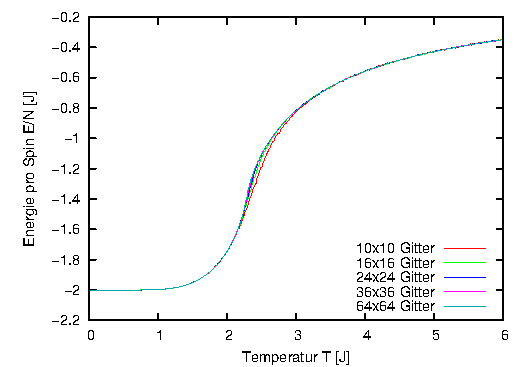
\includegraphics[width=0.48\textwidth]{Diagrams/KMCS/Energy-Temperature} 
  }
  \subfloat[{\bfseries Mittelwerte der W�rmekapazit�t}]{
    \label{fig:KMCSWaermekapazitaet}
    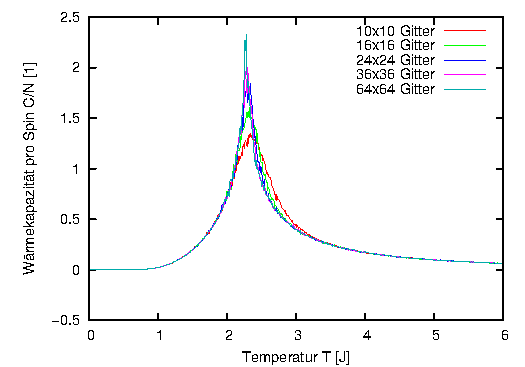
\includegraphics[width=0.48\textwidth]{Diagrams/KMCS/SpecificHeat-Temperature} 
  }
  \caption[Mittelwerte der Energie und W�rmekapazit�t; {\itshape Quelle:} Eigenwerk]{Mittelwerte der Energie und W�rmekapazit�t f�r verschieden gro�e Gitter mit periodischen Randbedingungen bei 10000 Messpunkten pro Temperaturpunkt; {\itshape Quelle:} Eigenwerk}
  \label{fig:KMCSEnergieWaermekapazitaet}
\end{figure}

Der Mittelwert der {\bfseries Energie} (Gl. \ref{eq:Energie}) in Abb. \ref{fig:KMCSEnergie} verl�uft erwartungsgem�� von -2 nach 0: F�r kleine Temperaturen stehen alle Spins in die gleiche Richtung ({\itshape Grundzustand}), da die Wahrscheinlichkeit eines Flips (Gl. \ref{eq:Gewicht}) eines einzelnen Spins gegen alle anderen verschwindend gering ist. Weil in einem 2-dimensionalen Gitter mit periodischen Randbedingungen die Anzahl der Koppelungen $N_b=2N$ ist, hat der Mittelwert hier den Wert -2. Je h�her jedoch die Temperatur steigt, je geringer wird der Einfluss des Boltzmann-Gewichts und f�hrt letztendlich zu einer Gleichverteilung der Spins, die f�r $T\rightarrow\infty$ $\left\langle E/N\right\rangle\rightarrow0$ liefert ({\itshape thermisches Chaos}).

Am Mittelwert der {\bfseries W�rmekapazit�t} (Gl. \ref{eq:Waermekapazitaet}) in Abb. \ref{fig:KMCSWaermekapazitaet}, also der Ableitung der mittleren Energie nach $T$, erkennt man deutlich den Phasen�bergang, der sich durch den h�chsten Wert f�r die Steigung der mittleren Energie erkenntlich macht. Dies erkl�rt sich durch die Bildung von gleichartig ausgerichteten (korrelierten) Spin-Clustern (Wei�sche Bezirke) in der Gr��enordnung der Korrelationsl�nge $\xi$ \cite{Nolting}. Da die Gr��e au�erdem die Varianz der Energie darstellt, erkl�rt sich der Verlauf ebenfalls aus der starken Reaktion der Energie auf geringste Temperatur�nderungen; hingegen sind Grundzustand und thermisches Chaos weitgehend "`stabil"'.

Ein Vergleich {\bfseries verschiedener Systemgr��en} zeigt eine Verschiebung des Peaks der mittleren W�rmekapazit�t als auch dessen Anwachsen, w�hrend abseits des Phasen�bergangs kein Unterschied festzustellen ist. Der Grund hierf�r kann wieder mit den Wei�schen Bezirken plausibel gemacht werden (siehe Seite 33 in \cite{Sandvik}):

\begin{itemize}
	\item $T\ll T_c$: Nahe am Grundzustand erwarten wir unabh�ngig von der Systemgr��e einen $\infty$-gr��en Bezirk mit vereinzelten St�rungen ($\xi=\infty$).
	\item $T\gg T_c$: Im thermischen Chaos ($\xi$ klein) von gr��tenteils dekorrelierten Einzelspins spielt die makroskopische Systemgr��e $N$ keine Rolle.
	\item $T\approx T_c$: Nahe dem Phasen�bergang nimmt jeder Bezirk einen makroskopischen Anteil des Systems ein, sodass sich das Verhalten bereits bei kleinen �nderungen massiv �ndert.
\end{itemize}

Um schlie�lich die reale �bergangstemperatur $T_c$ f�r $N\rightarrow\infty$ (thermodynamischer Limes) zu finden und die kritischen Exponenten bestimmen zu k�nnen, m�ssen wir einen polynominalen Fit �ber mehrere Systemgr��en hinweg verwenden (Finite Size Scaling) \cite{Buch}. F�r die obige Simulation ergab sich:

\begin{table}[htb]
	\centering
  \begin{tabular}{|l|l|l|l|}
    \hline
  	         & Eigene Werte & Exakter Wert & Wert durch Molekularfeldn�herung \\
    \hline
    $T_c$    & 2.26228      & 2.269185     & {\itshape Kein Wert} \\
    $\nu$    & 1            & 1            & 0.5 \\
    $\gamma$ & 1.75958      & 1.75         & 1   \\
    $\beta$  & 0.125        & 0.125        & 0.5 \\
    \hline
	\end{tabular}
	\caption{�bergangstemperatur und kritische Exponenten}
	\label{tab:kritischeexponenten}
\end{table}

\subsection{Autokorrelationszeit der Energie}

Wie wir sehen, nimmt auch die {\bfseries Autokorrelationszeit der Energie} $\tau_E$ (Gl. \ref{eq:Autokorrelationszeit}) in Abb. \ref{fig:KMCSAutokorrelationszeitEnergie} um den Phasen�bergang herum stark zu. Das bedeutet, dass die Konfigurationen �ber mehrere MC-Schritte hinweg korrelieren bzw. statistisch abh�ngig sind. Begr�ndet liegt dies in der Tatsache, dass die Korrelationsl�nge $\xi$ -- wie schon mehrfach erw�hnt -- am Phasen�bergang divergiert und die makroskopische Propagation von Information durch das System viel Zeit ben�tigt \cite{Buch}. $\tau_E$ ist neben der Temperatur auch vom System insbesondere dessen Gr��e abh�ngig.

\begin{figure}
  \centering
  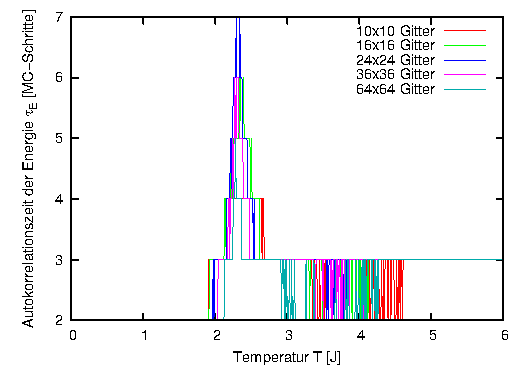
\includegraphics[width=0.48\textwidth]{Diagrams/KMCS/AutocorrelationtimeEnergy-Temperature} 
  \caption[Autokorrelationszeiten der Energie; {\itshape Quelle:} Eigenwerk]{{\bfseries Autokorrelationszeiten der Energie} f�r verschieden gro�e Gitter mit periodischen Randbedingungen bei 10000 Messpunkten pro Temperaturpunkt; {\itshape Quelle:} Eigenwerk}
  \label{fig:KMCSAutokorrelationszeitEnergie}
\end{figure}

\subsection{Mittelwert der Magnetisierung und magnetischen Suszeptibilit�t}

\begin{figure}[bh]
  \centering
  \subfloat[{\bfseries Mittelwerte der Magnetisierung}]{
    \label{fig:KMCSMagnetisierung}
    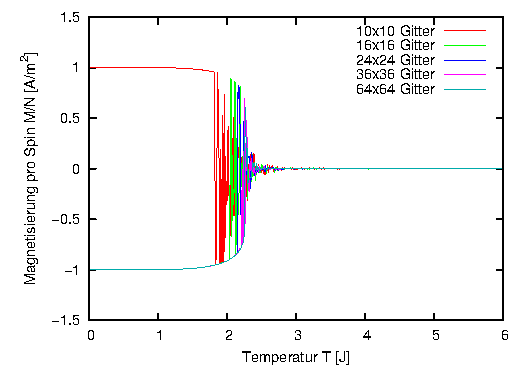
\includegraphics[width=0.48\textwidth]{Diagrams/KMCS/Magnetization-Temperature} 
  }
  \subfloat[{\bfseries Mittelwerte der mag. Suszeptibilit�t}]{
    \label{fig:KMCSSuszeptibilitaet}
    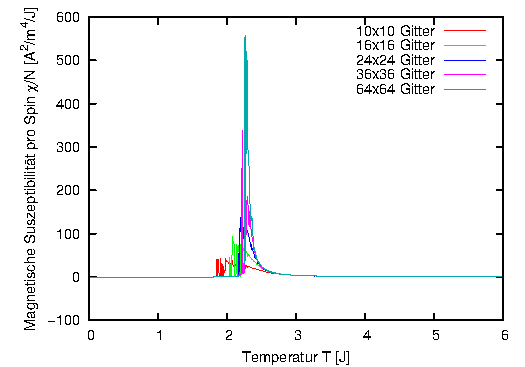
\includegraphics[width=0.48\textwidth]{Diagrams/KMCS/MagneticSusceptibility-Temperature} 
  }
  \caption[Mittlere Magnetisierung und magnetische Suszeptibilit�t; {\itshape Quelle:} Eigenwerk]{Mittlere Magnetisierung und magnetischen Suszeptibilit�t f�r verschieden gro�e Gitter mit periodischen Randbedingungen bei 10000 Messpunkten pro Temperaturpunkt; {\itshape Quelle:} Eigenwerk}
  \label{fig:KMCSMagnetisierungUndSuszeptibilitaet}
\end{figure}

Die weiter oben angesprochene (dekorrelierte) Gleichverteilung der Spins bei hohen Temperaturen, dr�ckt sich verst�ndlicherweise in der verschwindenen, mittleren {\bfseries Magnetisierung} (Gl. \ref{eq:Magnetisierung}) in Abb. \ref{fig:KMCSMagnetisierung} f�r $t\gg T_c$ aus. Verringert man vom thermischen Chaos aus die Temperatur, so beginnen die Spins in der N�he des kritischen Punktes, sich innerhalb der Wei�schen Bezirke in eine Richtung auszurichten. Da hierbei keine der beiden Richtungen einen Vorzug erh�lt, wechselt der Mittelwert der Magnetisierung beliebig das Vorzeichen.

Hier zeigt sich die Simulation mit dem Metropolis Algorithmus (Gl. \ref{eq:KanonischerMetropolis}) fehlerbehaftet, da sich die positiven und negativen Beitr�ge dieser Bezirke aus Symetriegr�nden insgesamt aufheben m�ssten. Die Cluster kann der {\bfseries Algorithmus} jedoch nur von den R�ndern her umdrehen, denn das Flippen eine Spins in der Mitte eines solchen Clusters ist sehr unwahrscheinlich. Die Cluster bleiben also f�r l�ngere Zeit bestehen und brechen die Symetrie der Verteilung -- es entsteht eine {\bfseries vermeintliche Magnetisierung}, die letztlich dem Verlust von Ergodizit�t (siehe Abschnitt \ref{sec:Ergodizitaet}) der Markov-Kette geschuldet ist. F�r kleine Temperaturen sieht man sogar, dass sich das Vorzeichen garnicht mehr ver�ndert und mit der Zeit alle Spins ebenfalls passend geflippt werden.

Ein Beispiel f�r eine Modifikation des Algorithmus', welcher diesem Sachverhalt Sorge tr�gt, ist der Cluster-Algorithmus, der von Swendson/Wang (1987) und Wolff (1989)  erstmals vorgestell wurde. Die Cluster werden analysiert, im Ganzen gewichtet und eventuell geflippt. F�r kleine Temperaturen werden die Cluster also korrekterweise ebenfalls bei fast jedem MC-Schritt geflippt und die Mittelung ergibt wie erwartet eine verschwindende Magnetisierung (vgl. \cite{Diplom}).

Die mittlere magnetische Suszeptibilit�t (Gl. \ref{eq:Suszeptibilitaet}) in Abb. \ref{fig:KMCSSuszeptibilitaet} zeigt ein �hnliches Verhalten, wie die W�rmekapazit�t. Auch sie formt zum Phasen�bergang hin einen einen Peak aus. In der Realit�t ist allerdings auch sie immer 0, falls es kein �u�eres Magnetfeld gibt.

\subsection{Mittelwert der abs. Magnetisierung und mag. Suszeptibilit�t}

Nachdem die Magnetisierung zuf�llig das Vorzeichen wechselt und sich f�r Systeme ohne externes Magnetfeld wegmittelt, betrachtet man h�ufig nur die {\bfseries absolute Magnetisierung} (Gl. \ref{eq:AbsoluteMagnetisierung}) in Abb. \ref{fig:KMCSAbsoluteMagnetisierung} und deren Varianz (Gl. \ref{eq:AbsoluteSuszeptibilitaet}) in Abb. \ref{fig:KMCSAbsoluteSuszeptibilitaet}. Beide Gr��en stellen sogenannte {\bfseries Ordnungsparameter} dar; sie verdeutlichen gut das Ausbilden von Clustern. Insbesondere zeigen sie f�r {\bfseries verschiedene Systemgr��en} $N$, dass der Prozess vom thermischen Chaos zur Ordnung hin im gr��eren System deutlich schneller vonstatten geht. Da sie Spin-Inversions-invariant sind, stellen sie trotz Clusterbildung Gr��en dar, welche der Metropolis Algorithmus zuverl�ssig berechnet.

Die mittlere absolute magnetische Suszeptibilit�t bietet sich neben der W�rmekapazit�t weiterhin an, $T_c$ und kritische Exponenten zu finden \ref{sec:IsingEnergie}.

\begin{figure}[bh]
  \centering
  \subfloat[{\bfseries Mittelwerte der abs. Magnetisierung}]{
    \label{fig:KMCSAbsoluteMagnetisierung}
    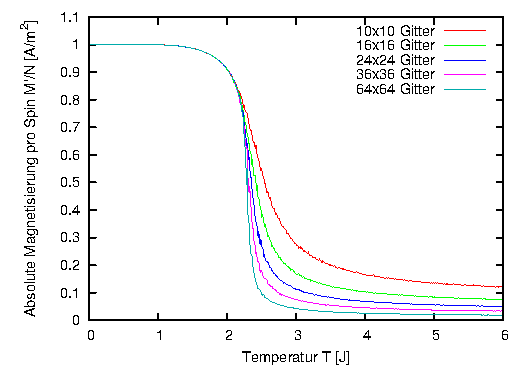
\includegraphics[width=0.48\textwidth]{Diagrams/KMCS/AbsoluteMagnetization-Temperature} 
  }
  \subfloat[{\bfseries Mittelwerte der abs. mag. Suszeptibilit�t}]{
    \label{fig:KMCSAbsoluteSuszeptibilitaet}
    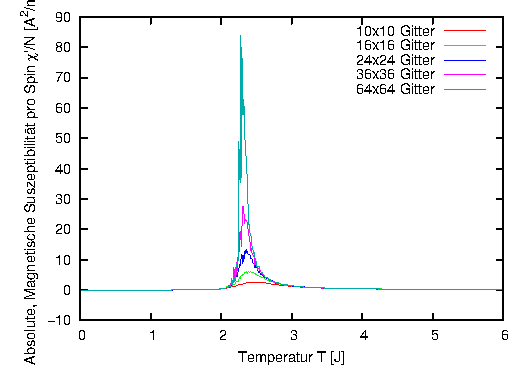
\includegraphics[width=0.48\textwidth]{Diagrams/KMCS/AbsoluteMagneticSusceptibility-Temperature} 
  }
  \caption[Mittlere abs. Magnetisierung und mag. Suszeptibilit�t; {\itshape Quelle:} Eigenwerk]{Mittelwerte der absoluten Magnetisierung und magnetischen Suszeptibilit�t f�r verschieden gro�e Gitter mit periodischen Randbedingungen bei 10000 Messpunkten pro Temperaturpunkt; {\itshape Quelle:} Eigenwerk}
  \label{fig:KMCSAbsoluteMagnetisierungUndSuszeptibilitaet}
\end{figure}

\newpage
\thispagestyle{empty}
\cleardoublepage
\chapter[Quantenmechanische MCS mit Hilfe der Stochastic Series Expansion]{Quantenmechanische MCS\\\LARGE mit Hilfe der Stochastic Series Expansion}
\label{sec:SSE}

Im Folgenden wollen wir uns nun der Simulation des quantenmechanischen Spin-1/2 Heisenberg Systems mithilfe der SSE nach \cite{Buch} und \cite{Sandvik} zuwenden. 

Unsere Beispielapplikation berechnet f�r verschiedene Systeme ({\itshape Offene Kette}, {\itshape Periodische Kette} und {\itshape Periodisches Gitter}) die Energie und die W�rmekapazit�t, wobei wir s�mtliche Daten immer entweder im Vergleich zur {\itshape Exakten Diagonalisierung} des Hamiltonoperators oder entsprechenden Literaturwerten betrachten und einordnen.

\section{Methode}

\subsection{Das Spin-1/2 Heisenberg System}

Der Hamiltonian des Spin-1/2 Heisenberg Systems mit Zeemann-Term ist gegeben durch:

\begin{equation}
H_{\mathrm{Heisenberg}}=\sum_{\left\langle i,j\right\rangle}J_{ij}\cdot\left(S_i^xS_j^x+S_i^yS_j^y+\Delta S_i^zS_j^z\right)-h\sum_{i=0}^{N-1}\mu_{i}\cdot S_i^z
\label{eq:HeisenbergHamiltonian}
\end{equation}

Man betrachtet also eine magnetische Koppelung von 3-dimensionalen, benachbarten Spins (abweichend in $Z$-Richtung um den Faktor $\Delta$) mit der Bindungsmatrix $\boldsymbol{J}$, an denen zus�tzlich ein externes Magnetfeld $\boldsymbol{h}=(0,0,h)^T$ angreift. Das magnetische Moment sei mit $\boldsymbol{\mu}=(0,0,\mu)^T$ benannt.

Das Heisenberg System wird folgenderma�en durch das $\Delta$ klassifiziert:

\begin{itemize}
\item $\Delta<-1$: Ising-Phase
\item $\Delta=-1$: Isotrope ferromagnetische Phase
\item $\vert\Delta\vert<1$: XY-Phase
\item $\Delta=1$: Isotrope antiferromagnetische Phase
\item $\Delta>1$: N\'eel-Phase
\end{itemize}

Wir wollen uns hier speziell mit der isotropen antiferromagnetischen Phase besch�ftigen, wobei wir auch hier wieder alle $J_{ij}=1$ sowie $\mu_i=1$ setzen wollen (Homogenit�t). Die Anordnung betrachten wir weiterhin ohne Magnetfeld ($h=0$). Daraus ergibt sich der vereinfachte Hamiltonian

\begin{equation}
H=\sum_{\left\langle i,j\right\rangle}S_i^xS_j^x+S_i^yS_j^y+S_i^zS_j^z=\sum_{\left\langle i,j\right\rangle}\boldsymbol{S}_i\cdot\boldsymbol{S}_j
\label{eq:BeispielHeisenbergHamiltonian}
\end{equation}

welchen man mit $S_i^\pm=S_i^x\pm iS_i^y$ zu

\begin{equation}
H=\sum_{b=1}^{N_b}\frac{1}{2}\left(S_{i(b)}^+S_{j(b)}^-+S_{i(b)}^-S_{j(b)}^+\right)+S_{i(b)}^zS_{j(b)}^z
\label{eq:BeispielHeisenbergHamiltonianPM}
\end{equation}

umformen kann, wobei wir die P�rchen $\left\langle i,j\right\rangle$ mit einem Index $b$ durchnummerieren und f�r die Spin-Indizes Nachbar-Funktionen $i(b)$ und $j(b)$ einf�hren; diese ergeben sich aus der Geometrie des Systems. Betrachtet man die Spin Operatoren dann in der Standardbasis bez�glich $S^z$, so kann man den Hamiltonian pro Koppelung (engl. Bond) in einen diagonalen $H_{0,b}$ und einen off-diagonalen Teil $H_{1,b}$ aufspalten:

\begin{equation}
H=-\sum_{b=1}^{N_b}\left(\underbrace{\frac{1}{4}-S_{i(b)}^zS_{j(b)}^z}_{H_{0,b}}-\underbrace{\frac{1}{2}\left(S_{i(b)}^+S_{j(b)}^-+S_{i(b)}^-S_{j(b)}^+\right)}_{H_{1,b}}\right) + \left\{\frac{N_b}{4}\right\}
\label{eq:BeispielHeisenbergHamiltonianTeile}
\end{equation}

Hierbei f�gen wir $H_{0,b}$ eine zus�tzliche Konstante $1/4$ ein, um die Eigenwerte des Produktoperators $-S_{i(b)}^zS_{j(b)}^z$ von $\pm1/4$ auf $\{0,\;1/2\}$, was f�r sp�tere Berechnungen bequemer ist.

\subsection{Reihenentwicklung}

Wie beim klassischen Ising Modell im Abschnitt \ref{sec:KlassischesSampling} versuchen wir nun auch, die Zustandssumme durch einen Monte-Carlo Ansatz anzun�hern, anstatt den gesamten Zustandsraum abtasten zu m�ssen. Der obere Ansatz ist hier jedoch nicht hilfreich, weil wir die Energie bzw. den Hamiltonian f�r den Boltzmannfaktor (in der Zustandssumme) nicht berechnen k�nnen. Deshalb schlagen wir einen anderen Weg ein:

Die quantenmechanische Zustandssumme

\begin{equation}
Z=\tr e^{-\beta H}
\label{eq:QuantenmechanischeZustandssumme}
\end{equation}

ist �ber Spur des "`Boltzmann-Operators"' definiert. Schreiben wir die Spur mit der Basis $\vert\alpha\rangle$ und verwenden f�r die Exponentialfunktion die Reihendarstellung, ergibt sich

\begin{align}
Z&=\sum_{n=0}^\infty\frac{(-\beta)^n}{n!}\sum_\alpha\langle\alpha\mid H^n\mid\alpha\rangle\label{eq:QuantenmechanischeZustandssummeReihe}\\
&=\sum_{n=0}^\infty\frac{(-\beta)^n}{n!}\sum_\alpha\langle\alpha\mid\left(-\sum_{b=1}^{N_b}H_{0,b}-H_{1,b}\right)^n\mid\alpha\rangle\label{eq:QuantenmechanischeZustandssummeHEingesetzt}\ \mathrm{,}
\end{align}

wobei wir die obige Gl. \ref{eq:BeispielHeisenbergHamiltonianTeile} f�r den Hamiltonian einsetzen.

An dieser Stelle f�hren wir die Potenzierung der Hamiltonians explizit durch Ausmultiplizieren aus und erhalten dadurch Hamiltonoperatorketten der L�nge $n$, sogenannte Operatorstrings. Jedes Kettenglied ist hierbei entweder diagonal oder off-diagonal und geh�rt zu einer bestimmten Koppelung $\langle i,j\rangle$ mit Index $b$. Da jede m�gliche Kombination von $n$ Operatoren vorkommt, haben wir insgesamt $(2N_b)^n$ Operatorstrings. Um diese geeignet zu verwalten, definieren wir die Menge aller Operatorstrings der L�nge $n$ als $\{S_n\}$ und ordnen jedem String je eine Funktion f�r die beiden Indizes $a(p)\in\{0,1\}$ und $b(p)\in\{1,\ldots,N_b\}$ der Hamiltonoperatoren zu, welche den exakten Operator $H_{a(p),b(p)}$ an der Position $p$ im String darstellen. Dar�ber hinaus hebt sich das erste Minuszeichen vor der Summe mit dem vor dem $\beta$ weg und das Minuszeichen zwischen den Hamiltonoperatoren ziehen wir mit der Anzahl der off-diagonalen Operatoren $n_1$ vor das Matrixelement:

\begin{equation}
Z=\sum_{n=0}^\infty\frac{\beta^n}{n!}\sum_\alpha\sum_{\{S_n\}}(-1)^{n_1}\langle\alpha\mid\prod_{p=0}^{n-1}H_{a(p),b(p)}\mid\alpha\rangle
\label{eq:QuantenmechanischeZustandssummeStrings}
\end{equation}

Nun betrachten wir noch die unendliche Summe �ber $n$. Diese schneiden wir bei $n=L$ ab (eine Fehlerrechnung folgt sp�ter) und bringen alle Operatorstrings mit $n<L$ auf die L�nge $L$, indem wir $L-n$ Einheitsmatrizen in sie einf�gen, die wir sinnvollerweise $H_{0,0}$ nennen. Dies f�hrt zu nur noch {\bfseries einer} Menge von Operatorstrings $S_L$, in die die k�rzeren integriert wurden. Da es aber $\binom{L}{n}$ M�glichkeiten gibt die Einheitsmatrizen einzuf�gen, m�ssen wir zus�tzlich durch diese Vielfachheit teilen, da ein ehemaliger $S_n$ Operatorstring auch zuk�nftig nur einfach in die Zustandssumme eingehen soll:

\begin{equation}
Z=\sum_{\{S_L\}}\frac{\beta^{n}(-1)^{n_1}(L-n)!}{L!}\sum_\alpha\langle\alpha\mid\prod_{p=0}^{L-1}H_{a(p),b(p)}\mid\alpha\rangle
\label{eq:QuantenmechanischeZustandssummeAbschneiden}
\end{equation}

$n$ ist nun nicht mehr die Stringl�nge, sondern die Anzahl der Operatoren ungleich $H_{0,0}$.

Wir wollen nun die Wirkung des Operatorstrings auf die Basis $\vert\alpha\rangle$ betrachten: Diese {\itshape propagierten Zust�nde}

\begin{equation}
\vert\alpha(Q)\rangle=\prod_{p=0}^{Q-1}H_{a(p),b(p)}\mid\alpha\rangle
\label{eq:PropagierteZust�nde}
\end{equation}

sind neue Basiszust�nde, sie ergeben sich also nicht aus der Superposition von anderen Zust�nden. Explizit ist die Wirkung eines diagonalen Operators auf einen Basiszustand

\begin{align}
H_{0,b}\mid\ldots\uparrow_{i(b)}\ldots\uparrow_{j(b)}\ldots\rangle&=\frac{1}{4}-(\frac{1}{2}\cdot\frac{1}{2})=0\ \mathrm{,}\label{eq:DigonalOpAuf11}\\
H_{0,b}\mid\ldots\downarrow_{i(b)}\ldots\downarrow_{j(b)}\ldots\rangle&=\frac{1}{4}-(-\frac{1}{2}\cdot-\frac{1}{2})=0\ \mathrm{,}\label{eq:DigonalOpAuf00}\\
\langle\ldots\uparrow_{i(b)}\ldots\downarrow_{j(b)}\ldots\mid H_{0,b}\mid\ldots\uparrow_{i(b)}\ldots\downarrow_{j(b)}\ldots\rangle&=\frac{1}{4}-(\frac{1}{2}\cdot-\frac{1}{2})=\frac{1}{2}\ \mathrm{,}\label{eq:DigonalOpAuf10}\\
\langle\ldots\downarrow_{i(b)}\ldots\uparrow_{j(b)}\ldots\mid H_{0,b}\mid\ldots\downarrow_{i(b)}\ldots\uparrow_{j(b)}\ldots\rangle&=\frac{1}{4}-(-\frac{1}{2}\cdot\frac{1}{2})=\frac{1}{2}\label{eq:DigonalOpAuf01}
\end{align}

und die Wirkung eines off-diagonalen Operators auf einen Basiszustand

\begin{align}
H_{1,b}\mid\ldots\uparrow_{i(b)}\ldots\uparrow_{j(b)}\ldots\rangle&=\frac{1}{2}(0+0)=0\ \mathrm{,}\label{eq:OffDigonalOpAuf11}\\
H_{1,b}\mid\ldots\downarrow_{i(b)}\ldots\downarrow_{j(b)}\ldots\rangle&=\frac{1}{2}(0+0)=0\ \mathrm{,}\label{eq:OffDigonalOpAuf00}\\
\langle\ldots\downarrow_{i(b)}\ldots\uparrow_{j(b)}\ldots\mid H_{0,b}\mid\ldots\uparrow_{i(b)}\ldots\downarrow_{j(b)}\ldots\rangle&=\frac{1}{2}\ \mathrm{,}\label{eq:OffDigonalOpAuf10}\\
\langle\ldots\uparrow_{i(b)}\ldots\downarrow_{j(b)}\ldots\mid H_{0,b}\mid\ldots\downarrow_{i(b)}\ldots\uparrow_{j(b)}\ldots\rangle&=\frac{1}{2}\ \mathrm{.}\label{eq:OffDigonalOpAuf01}
\end{align}

Dieser Sachverhalt vereinfacht den Algorithmus deutlich. Beim sp�teren Sampling tragen also nur solche Operatorstrings bei, deren Operatoren auf nicht-parallele Spins wirken. Das Matrixelement einer solchen Operation ist au�erdem immer $\frac{1}{2}$ (dies war der Grund f�r die Konstante $1/4$ in $H_{0,b}$ aus Gl. \ref{eq:BeispielHeisenbergHamiltonianTeile}).

Das Gewicht f�r eine beitragende Konfiguration $\sigma$ ist also

\begin{equation}
p(\sigma,S_L)=\left(\frac{\beta}{2}\right)^n\frac{(L-n)!}{L!}
\label{eq:HeisenbergGewichte}
\end{equation}

wobei wir verwenden, dass $n_1$ auf Quadratgittern und Ketten immer gerade ist und deshalb wegf�llt \cite{Sandvik}.

\subsection{Sampling}

Wir wenden nun die {\bfseries Monte-Carlo Methode} auf Operatorstrings anstatt Zust�nden an: Zu Beginn der Simulation gehen wir von einem leeren Operatorstring und einer zuf�lligen Spinanordnung aus und f�hren wie in Kapitel \ref{sec:Ising} MC-Schritte aus. Diese sind unterteilt in ein Diagonal Update, welches diagonale Operatoren in den String ein- und ausbaut und in ein so genanntes off-diagonales Loop Update, welches diagonale zu off-diagonale Operatoren hin- und zur�cktransformiert. Jedes Update muss allerdings darauf achten, dass die oben angegeben Beschr�nkungen nicht verletzt werden:

\begin{itemize}
\item Operatoren d�rfen nicht auf parallele Spin-Paare wirken, ansonsten annihilieren sie den Zustand (lokale Bedingung).
\item Die Periodizit�t $\vert\alpha\rangle=\vert\alpha(0)\rangle=\vert\alpha(L)\rangle$ des Algorithmus' muss gewahrt werden.
\end{itemize}

Das Sampling kann durch Graphiken wie \ref{fig:OffDiagonalNormal} veranschaulicht werden. Die Anfangskonfiguration $\vert\alpha(0)\rangle$ steht hierbei unten und propagiert durch den Operatorstring in den Endzustand $\vert\alpha(L)\rangle=\vert\alpha(0)\rangle$. Operatoren sitzen jeweils auf zwei "`Spin-Bahnen"' und lassen diese entweder unber�hrt (diagonale Operatoren, wei� dargestellt) oder vertauschen deren Ausrichtung (off-diagonale Operatoren, schwarz dargestellt). Reihen ohne Operatoren signalisieren einen $H_{0,0}$ Operator, also eine Einheitsmatrix.

\begin{figure}[thb]
  \centering
  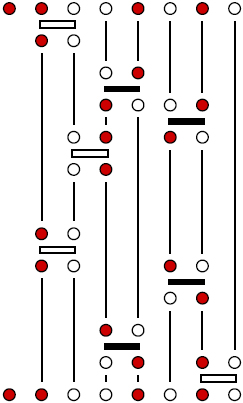
\includegraphics[width=0.3\textwidth]{Images/Off-Diagonal-Normal} 
  \caption[Visualisierung des Operatorstrings; {\itshape Quelle:} \cite{Sandvik}]{{\bfseries Visualisierung des Operatorstrings:} Die Kreise ganz unten und ganz oben stellen die Spinkonfiguration $\vert\alpha(0)\rangle$ bzw. $\vert\alpha(L)\rangle$ dar. Dazwischen liegen diagonale (wei�) und off-diagonale Operatoren (schwarz). Reihen ohne Operatoren signalisieren einen $H_{0,0}$ Operator; {\itshape Quelle:} \cite{Sandvik}}
  \label{fig:OffDiagonalNormal}
\end{figure}

\subsubsection{Diagonales Update}

F�r das Einf�gen von diagonalen Operatoren in den String muss darauf geachtet werden, dass dieser nicht an parallele Spins angelegt wird. Die Periodizit�t hingegen wird durch die Aktion nicht gest�rt, da diagonale Operatoren den Zustand nicht ver�ndern. Das Entfernen von diagonalen Operatoren aus dem Operatorstring ist generell unproblematisch.

Wir legen nun unsere �bergangswahrscheinlichkeiten $\boldsymbol{W}$ f�r das Einf�gen eines Operators an einem Platz $p$ gem�� des {\bfseries Metropolis Algorithmus'} fest (Gl. \ref{eq:Metropolis}):

\begin{equation}
W_{\nu\sigma,\ \mathrm{Einf"ugen}}=\begin{cases}
\frac{p(\sigma,S_L)\cdot N_b}{p(\nu,S_L)}=\frac{\beta N_b}{2(L-n)} & p(\sigma,S_L)\cdot N_b<p(\nu,S_L)\\
1                                                                  & p(\sigma,S_L)\cdot N_b\geq p(\nu,S_L)
\end{cases}
\label{eq:EinfuegeWahrscheinlichkeit}
\end{equation}

Analog erh�lt man beim L�schens eines Operators (ersetzen mit der Einheitsmatrix)

\begin{equation}
W_{\nu\sigma,\ \mathrm{Entfernen}}=\begin{cases}
\frac{p(\sigma,S_L)\cdot N_b}{p(\nu,S_L)}=\frac{2(L-n+1)}{\beta N_b} & p(\sigma,S_L)\cdot N_b<p(\nu,S_L)\\
1                                                                    & p(\sigma,S_L)\cdot N_b\geq p(\nu,S_L)\ \mathrm{.}
\end{cases}
\label{eq:EntferneWahrscheinlichkeit}
\end{equation}

Die Eigenschaft {\itshape Detailed Balance} kann sofort durch Einsetzen in \ref{eq:DetailedBalance} verifiziert werden.

\subsubsection{Off-Diagonales Loop Update}

Beim Austausch von diagonalen und off-diagonalen Operatoren ist der Sachverhalt etwas komplizierter, denn dadurch wird ein Vertauschen von Spinrichtungen (durch den off-diagonalen Operator) hinzugef�gt bzw. entfernt. Es ist selbstverst�ndlich, dass unter der Ber�cksichtigung der Periodizit�t also mindestens zwei off-diagonale Operatoren in solch eine Aktion involviert sein m�ssen. Befinden sich zwischen diesem Operator-Paar allerdings weitere Operatoren, kann es zu einer Regelverletztung der lokalen Bedingung kommen, da ein �ndern der Zust�nde zwischen dem Operatorpaar den dazwischen liegenden beeinflusst (siehe Abb. \ref{fig:Off-Diagonal-Works}). In Abb. \ref{fig:Off-Diagonal-NeedsLoop} wird eine m�gliche L�sung dieses Problems dargestellt; hierbei wird nicht der Zustand zwischen dem Operatorenpaar ver�ndert, sondern der au�erhalb (inklusive dem Anfangs- und Endzustand).

\begin{figure}[thb]
  \centering
  \subfloat[{\bfseries Problematischer (gestrichelt) und Unproblematischer Fall (durchgezogen)}]{
    \label{fig:Off-Diagonal-Works}
    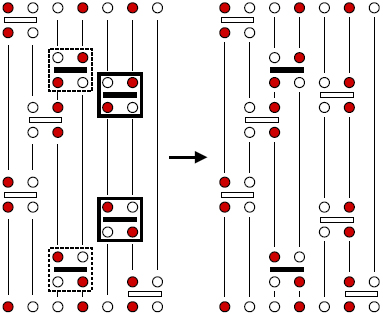
\includegraphics[width=0.41\textwidth]{Images/Off-Diagonal-Works} 
  }\quad\quad
  \subfloat[{\bfseries Ausweg �ber die Modifikation des Anfangszustand}]{
    \label{fig:Off-Diagonal-NeedsLoop}
    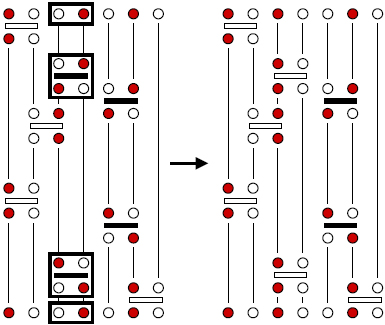
\includegraphics[width=0.41\textwidth]{Images/Off-Diagonal-NeedsLoop} 
  }
  \caption[M�gl. Probleme beim Off-Diagiagonalen Loop Update; {\itshape Quelle:} \cite{Sandvik}]{M�gliche Probleme bzgl. verletzte Bedingungen beim Off-Diagonalen Update. In (a) sehen wir, wie das durchgezogen marktierte Update unproblematisch durchgef�hrt, wobei das gestrichelte Update den Operator zwischen dem Paar so beeinflussen w�rde, dass dieser die lokale Bedingung nicht mehr erf�llt. In (b) sehen wir einen m�glichen Ausweg, da hier Zust�nde zwischen den Operatoren nicht ge�ndert werden, sondern der Anfangs- bzw. Endzustand; {\itshape Quelle:} \cite{Sandvik}}
  \label{fig:ProblematikVonOffDiagonalUpdates}
\end{figure}

Eine andere M�glichkeit w�re nat�rlich, den zweiten (links) anliegenden Spin des involvierten mittleren Operators auch zu �ndern, sodass die lokale Bedingung insgesamt wieder erf�llt ist. Dies beeinflusst aber wieder andere Operatoren, etc.. Im Endeffekt versucht man also, alle sogenannten Loops (siehe Abb. \ref{fig:Off-Diagonal-Loop}), d.h. abgeschlossene Wege durch den Operatorstring, zu finden, da man diese dann wie in Abb. \ref{fig:Off-Diagonal-LoopDone} unabh�ngig von einander flippen kann (Loop Update), wobei Operatoren die ganz in der Loop liegen hin- und sogleich wieder zur�ckgeflippt werden. Der Ausweg in Abb. \ref{fig:Off-Diagonal-NeedsLoop} ist in dieser L�sung inbegriffen, da Loops auch �ber den periodischen Rand hinaus f�hren k�nnen.

\begin{figure}[thb]
  \centering
  \subfloat[{\bfseries Operatorstring mit eingezeichneter Loop}]{
    \label{fig:Off-Diagonal-Loop}
    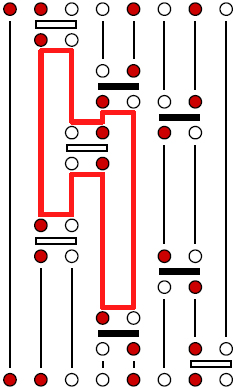
\includegraphics[width=0.3\textwidth]{Images/Off-Diagonal-Loop} 
  }\quad\quad
  \subfloat[{\bfseries Operatorstring nach dem Flippen der Loop}]{
    \label{fig:Off-Diagonal-LoopDone}
    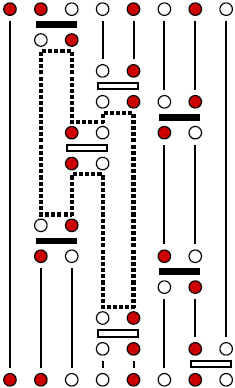
\includegraphics[width=0.3\textwidth]{Images/Off-Diagonal-LoopDone} 
  }
  \caption[Loop im Operatorstring; {\itshape Quelle:} \cite{Sandvik}]{Loop im Operatorstring. (a) bezieht sich noch auf den Ausgangszustand, (b) ergiebt sich nach dem flippen der in (a) angegeben Loop. Operatoren derer beider Seiten am selben Loop liegen werden nicht geflippt (hin und wieder zur�ckgeflippt); {\itshape Quelle:} \cite{Sandvik}}
  \label{fig:LoesungDurchLoopUpdate}
\end{figure}

\subsection{Formeln f�r die mittlere Energie und W�rmekapazit�t}

\subsubsection{Energie}

Augehend von der Gl. \ref{eq:QuantenmechanischeZustandssummeReihe} wollen wir nun eine Formel f�r die mittlere Energie pro Spin $E/N$ herleiten,

\begin{equation}
Z=\sum_{n=0}^\infty\frac{(-\beta)^n}{n!}\sum_{\{\alpha\}_n}\langle\alpha_0\mid H\mid\alpha_{n-1}\cdots\langle\alpha_1\mid H\mid\alpha_0\rangle\ \mathrm{,}
\label{eq:QuantenmechanischeZustandssummeReiheAusgeschrieben}
\end{equation}

wobei in die hintere Summe $n-1$ Summen �ber die Basis eingef�gt wurden. Sodann ergiebt sich der Mittelwert von $E/N$ mit:

\begin{align}
\allowdisplaybreaks
\frac{E}{N}&=\frac{1}{ZN}\sum_{n=0}^\infty\frac{(-\beta)^n}{n!}\sum_{\{\alpha\}_{n+1}}\langle\alpha_0\mid H\mid\alpha_n\cdots\langle\alpha_1\mid H\mid\alpha_0\rangle\label{eq:QuantenEnergie}\\
           &=\frac{1}{ZN}\sum_{n=1}^\infty\frac{(-\beta)^n}{n!}\frac{n}{-\beta}\sum_{\{\alpha\}_n}\langle\alpha_0\mid H\mid\alpha_{n-1}\cdots\langle\alpha_1\mid H\mid\alpha_0\rangle\label{eq:QuantenEnergieSubstitution}
           \displaybreak\\
           &=\frac{1}{ZN}\sum_{n=0}^\infty\frac{(-\beta)^n}{n!}\frac{n}{-\beta}\sum_{\{\alpha\}_n}\langle\alpha_0\mid H\mid\alpha_{n-1}\cdots\langle\alpha_1\mid H\mid\alpha_0\rangle\label{eq:QuantenEnergieMit0}\\
           &=-\frac{\langle n\rangle}{N\beta}\label{eq:QuantenEnergieMittelwert}\\
\left(\frac{E}{N}\right)_{\mathrm{Real}}&=-\frac{\langle n\rangle}{N\beta}+\left\{\frac{N_b}{4N}\right\}\label{eq:QuantenEnergieMitShift}
\end{align}

F�r die erste Gleichheit bemerken wir, dass die letzte Summe nun �ber ein $H$ mehr l�uft. Diese erste Umformung substituiert $n:=n+1$, die zweite f�gt den $n=0$-Term wieder ein, dies ist m�glich, da er ohnehin 0 ergibt. Sodann kann erkannt werden, dass es sich bei dem vorliegenden Ausdruck um den Mittelwert von $n$ handelt. Zu guter Letzt f�gen wir noch die "`verlorene"' Energie-Konstante von Gl. \ref{eq:BeispielHeisenbergHamiltonianTeile} hinzu.

\subsubsection{W�rmekapazit�t}

Die W�rmekapazit�t pro Spin erh�lt man dann �ber die Ableitung der mittleren Energie nach der Temperatur:

\begin{align}
\frac{C}{N}&=\frac{\partial_T E}{N}\\
           &=-\frac{1}{NT}\partial_T \langle n\rangle-\frac{\langle n\rangle}{N}\label{eq:QuantenWaermeKapazitaet}\\
           &=\frac{\langle n^2\rangle-\langle n\rangle^2-\langle n\rangle}{N}\label{eq:QuantenWaermeKapazitaetBest}
\end{align}

\subsection{Cut-Off L}
\label{sec:cutoff}

Da f�r $T\rightarrow\infty$ von $C\rightarrow0$ ausgegangen werden kann, sehen wir, dass $\var n=\langle n\rangle$, das hei�t, der $T$ -- $n$ Graph f�llt in beide Richtungen exponentiell ab. Nach \cite{Sandvik} kann f�r $L$ also ein hinreichend h�herer Wert als $\langle n\rangle$ verwendet werden (ca. $4/3\cdot\langle n\rangle$). Dann erreicht $n$ praktisch nie $L$.

Der Algorithmus muss $L$ also f�r jeden MC-Schritt �berpr�fen und gegebenfalls anpassen.

\section{Implementierung}

Die Struktur der Anwendung ist ebenfalls wieder eng angelehnt an die Beschreibung in \cite{Sandvik}. Der Algorithmus �hnelt dem der klassischen MCS in Abschnitt \ref{sec:KlassischeImplementierung} deutlich, verwendet allerdings andere Messformeln (Gl. \ref{eq:QuantenEnergieMitShift} und \ref{eq:QuantenWaermeKapazitaetBest}) und einen anderen MC-Schritt, da er den Operatorstring inklusive Anfangskonfiguration sampled und nicht nur einzelne Konfigurationen.

\subsection{Initialisierung}

Wie bei der klassischen MCS ben�tigen wir zuerst die Eingabeparameter:

\begin{itemize}
\item Anzahl der Spins $N$
\item Anzahl der Messungen $R_1$
\item Temperatur des Systems $T$
\end{itemize}

Anschlie�end legen wir wieder ein boolsches Array der L�nge $N$ an, welches unseren Anfangszustand $\vert\alpha(0)\rangle$ enth�lt, und initialisieren es mit zuf�lligen Werten. Um den aktuellen Operatorstring abspeichern zu k�nnen, legen wir weiterhin ein Integer-Array $s$ der L�nge $L$ an, welches f�r jeden Platz $p$ im String die Art des Operators (diagonal, off-diagonal oder Einheitsmatrix) -- also $a(p)$ und dessen Position im System $b(p)$ (Koppelung) speichert. Dies k�nnen wir gemeinsam in einer Ganzzahl speichern, wenn wir ausnutzen, dass $a\in\{0,1\}$:

\begin{equation}
s(p)=a(p)+2b(p)
\label{eq:OperatorArrayStorage}
\end{equation}

Wir k�nnen die Informationen aus der Ganzzahl $s(p)$ wieder erhalten, wenn wir pr�fen, ob

\begin{itemize}
\item $s(p)=0 \Rightarrow$ Einheitsmatrix,
\item $\even s(p) \Rightarrow$ Diagonaler Operator,
\item $\odd s(p) \Rightarrow$ Off-diagonaler Operator.
\end{itemize}

Die Position $b(p)$ des Operators erhalten wir, wenn wir mittels einer ganzzahligen Division $b(p)=s(p)/2$. Au�erdem speichern wir die Anzahl der Operatoren $n$, die nicht eine Einheitsmatrix darstellen, da diese Gr��e sp�ter zum Berechnen unserer Messgr��en verwendet wird.

\subsection{Simulation}

F�r jeden MC-Schritt wird zuerst ein Diagonal Update durchgef�hrt und anschlie�end ein Off-Diagonal Loop Update. Abschlie�end wird der Cut-Off $L$ nach Abschnitt \ref{sec:cutoff} eventuell weiter noch oben gesetzt, um dem System genug Freiraum zum Einf�gen weiterer Operatoren zu geben, d.h. wir verl�ngern den Operatorstring, um immer genug Einheitsmatrizen frei f�r diagonale Operatoren zu haben.

\subsubsection{Diagonal Update}

Bei jedem Diagonal Update wird f�r jeden Operatorplatz $p$, auf dem bereits ein diagonaler Operator sitzt, mittels einem Zufallstest entschieden, ob der Operator durch eine Einheitsmatrix ersetzt werden darf. Ist eine Zufallszahl kleiner als die Wahrscheinlichkeit aus Gl. \ref{eq:EntferneWahrscheinlichkeit}, verringert man $n$ um 1 und vermerkt im Operatorstring $s(p)=0$.

Existiert noch kein Operator auf der Position, versucht man einen diagonalen Operator einzuf�gen: Die Koppelung $b$ des Operators wird zuf�llig bestimmt. Wenn die beiden Spins an dieser Koppelung anti-parallel sind, wird mit einem �hnlichen Zufallstest wie oben mit der Wahrscheinlichkeit aus Gl. \ref{eq:EinfuegeWahrscheinlichkeit} entschieden, ob das Einf�gen erfolgt. Als Konsquenz w�rden wir $n$ um 1 erh�hen und $s(p)=2b$ setzen. Um den bis zu $p$ propagierten Zustand $\vert\alpha(p)\rangle$ schnell zu erhalten, schreiben wir ihn in jedem $p$-Schritt mit.

Trifft man auf einen Off-Diagonalen Operator, wird nichts am Operatorstring ver�ndert, lediglich der propagierte Zustand wird angepasst (die beiden Spins tauschen ihren Zustand).

\subsubsection{Off-Diagonal Loop Update}

Um nun die durch das Diagonal Update eingef�gten Operatoren auch in Off-Diagonale Operatoren zu transformieren (oder zur�ck), wird der Operatorstring nun systematisch nach Loops gescannt und f�r jeden Loop wird anschlie�end mit der Wahrscheinlichkeit von 50\% entschieden, diesen gesamten Loop zu flippen.

\paragraph{Die Analyse des Operatorstrings}

Jeder Operator (der keine Einheitsmatrix ist) besitzt vier Vertizes, welche die Ankn�pfungspunkte an die Spin-Bahnen (zwei oben, zwei unten) sind. Diese erhalten nach Abb. \ref{fig:Vertizes} je eine Typnummer $y\in\{0,1,2,3\}$. Mithilfe dieses $y$ und der Position des Operators im String $p$ kann man jeden Vertex global mit der Zahl $v$ indizieren:

\begin{equation}
v(y,p)=v+4p
\label{eq:OperatorVertexStorage}
\end{equation}

Von der Ganzzahl $v$ kann man wie bei \ref{eq:OperatorArrayStorage} wieder auf die speziellen Eigenschaften schlie�en.

\begin{figure}[thb]
  \centering
  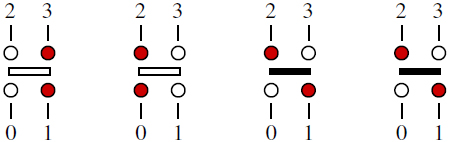
\includegraphics[width=0.4\textwidth]{Images/Vertizes}
  \caption[M�gliche Verwendung der Operatoren mit den Vertex-Typnummern; {\itshape Quelle:} \cite{Sandvik}]{{\bfseries M�gliche Verwendung der Operatoren mit den Typnummern der Vertizes}; {\itshape Quelle:} \cite{Sandvik}}
  \label{fig:Vertizes}
\end{figure}

Nun gehen wir jede Position $p$ im String durch und verkn�pfen Vertizes, die sich auf einer Spin-Bahn gegen�berliegen. Die Verkn�pfungen stellen also die dicken Linien dar, z.B. wie in Abb. \ref{fig:Off-Diagonal-Loop}, die die Operatoren verbinden. D.h. Vertizes stellen die Ecken eines Loop-Gebiets dar, diese Verkn�pfungen und die Operatoren die Kanten. Die Verkn�pfung wird in einem Verkn�pfungs-Array $x$ gespeichert. Zu beachten ist, dass Loops durchaus auch �ber den periodischen Rand hinweg m�glich sind!

\paragraph{Flippen der Loops}

Dieses wird nun St�ck f�r St�ck durchgef�hrt: F�r jede Loop wird mit einer Wahrscheinlichkeit 50\% entschieden, ob diese geflippt werden soll. Ist dies der Fall, geht man auf den Kanten des Loop-Gebiets von Operator zu Operator und flippt einen jeden. Operatoren, die mitten in einer Loop liegen, werden also nicht ver�ndert. Wird eine Loop geflippt, die sich �ber die periodischen R�nder hinaus erstreckt, muss anschlie�end der Anfangszustand demensprechend ver�ndert werden.

\subsection{Analyse}

Die abgespeicherten Werte f�r $n$ werden nach der Simulation verwendet, um sie -- wie in Abschnitt \ref{sec:Autokorrelation} erkl�rt -- zu analysieren. Ihre Anwendung zur Berechnung der Gr��en {\bfseries Energie} und {\bfseries W�rmekapazit�t} werden in den Gleichungen \ref{eq:QuantenEnergieMitShift} und \ref{eq:QuantenWaermeKapazitaetBest} beschrieben.

\subsection{Quellcode}

Der vom Author geschriebene C++ Quellcode ist im Anhang \ref{sec:code} zu finden. Folgende Dateien sind f�r diese quantenmechanische Simulation relevant:

\begin{itemize}
\item\ref{code:SIM}: Hauptprogramm SIM
\item\ref{code:AbstractLattice}: Abstrakte Gitterklasse
\item\ref{code:Open1DLattice}: 1D Kette mit offenen Randbedingungen
\item\ref{code:Periodic1DLattice}: 1D Kette mit periodischen Randbedingungen
\item\ref{code:Periodic2DLattice}: 2D Gitter mit periodischen Randbedingungen
\item\ref{code:AbstractAlgorithm}: Abstrakte Algorithmusklasse
\item\ref{code:SSEAlgorithm}: SSE Algorithmus
\item\ref{code:AbstractAnalyzer}: Abstrakte Analyseklasse
\item\ref{code:SseEnergyAnalyzer}: Analyse f�r die Energie (SSE)
\item\ref{code:SseHeatCapacityAnalyzer}: Analyse f�r die W�rmekapazit�t (SSE)
\end{itemize}

\section{Ergebnisse und Diskussion}

Im Folgenden sind die Messergebnisse der SSE-Simulationen aufgef�hrt. Bis auf die explizite Erw�hnung im ersten Unterabschnitt wurde auf eine Fehlerdarstellung in den Diagrammen verzichtet, da die Fehler ihrer (kleinen) Gr��e wegen nicht darstellbar waren.

\subsection{Heisenbergkette mit periodischen Randbedingungen}

Auf den Abbildungen \ref{fig:KettenEnergieTemperatur} und \ref{fig:KettenWaermekapazitaetTemperatur} sieht man die mittlere Energie und die mittlere W�rmekapazit�t f�r verschieden gro�e Systeme (periodische Ketten) aufgetragen. Diese Kurven verlaufen stets �bereinander, da im 1-dimensionalen Fall noch kein Phasen�bergang auftritt. Das System befindet sich also entweder nahe dem Grundzustand oder besitzt bereits eine so geringe Korrelationsl�nge, dass f�r verschiedene Gr��en keine Effekte auftreten (vgl. Er�rterung in \ref{sec:IsingEnergie}). Die jeweils gleiche Grundzustandsenergie von $-0.4432$ stimmt sehr gut mit dem in \cite{Diplom} auf Seite 58 angegeben Wert �berein.

\begin{figure}[bth]
  \centering
  \subfloat[{\bfseries Mittelwerte der Energie}]{
    \label{fig:KettenEnergieTemperatur}
    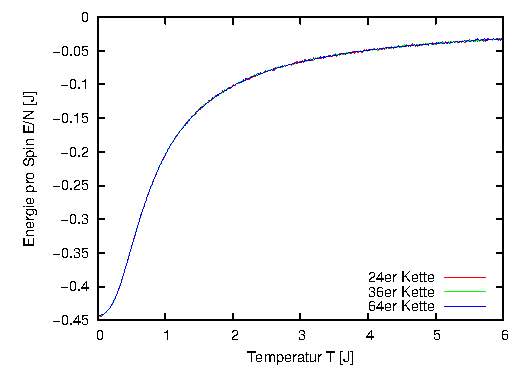
\includegraphics[width=0.48\textwidth]{Diagrams/SSE/Chain_Energy-Temperature} 
  }
  \subfloat[{\bfseries Mittelwerte der W�rmekapazit�t}]{
    \label{fig:KettenWaermekapazitaetTemperatur}
    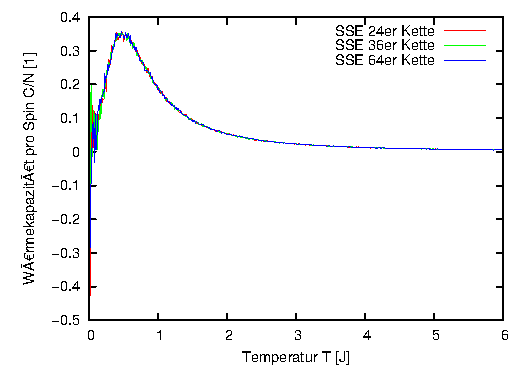
\includegraphics[width=0.48\textwidth]{Diagrams/SSE/Chain_SpecificHeat-Temperature} 
  }
  \caption[Mittelwerte der Energie und W�rmekapazit�t; {\itshape Quelle:} Eigenwerk]{Mittelwerte der Energie und W�rmekapazit�t f�r verschiedene Systemgr��en einer periodischen Kette bei 100000 Messpunkten pro Temperaturpunkt; {\itshape Quelle:} Eigenwerk}
  \label{fig:KettenEnergieWaermekapazitaet}
\end{figure}

Wir betrachten nun noch explizit den absoluten Fehler (Standardabweichung) in Abb. \ref{fig:KettenFehlerEnergie}: Mit steigender Systemgr��e tritt also ein immer st�rker Effekt zu Tage; bei hohen Temperaturen gibt es wesentlich mehr m�gliche Konfigurationen. All diese Konfigurationen haben eine �hnliche Energie und m�ssen gesampelt werden. Bei $T=0$ muss das System nur zum Grundzustand finden.

\begin{figure}
  \centering
  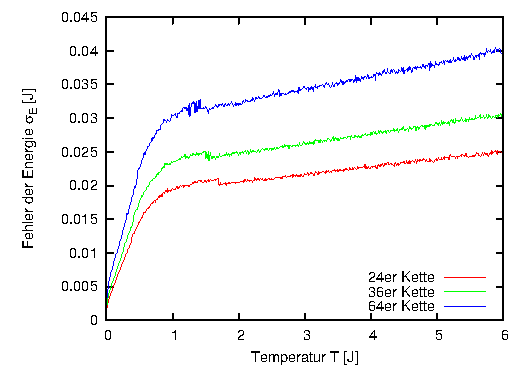
\includegraphics[width=0.48\textwidth]{Diagrams/SSE/Chain_ErrorEnergy-Temperature} 
  \caption[Absoluter Fehler der Energie; {\itshape Quelle:} Eigenwerk]{{\bfseries Absoluter Fehler der Energie} f�r verschiedene Systemgr��en einer periodischen Kette bei 100000 Messpunkten pro Temperaturpunkt; {\itshape Quelle:} Eigenwerk}
  \label{fig:KettenFehlerEnergie}
\end{figure}

\subsection{Heisenberggitter mit periodischen Randbedingungen}

Nach Korrolar 1.11 aus \cite{Branch} besitzt das 2-dimensionale Gitter im Gegensatz zum 1D-Fall einen Phasen�bergang, d.h. zur Temperatur $T_c$ hin divergiert die Korrelationsl�nge und damit die Gr��e der Wei�schen Bezirke (Cluster), so dass in der Umgebung um diesen kritischen Punkt die Gr��e des Systems eine gravierende Rolle spielt. Beide Grundzustandsenergien, -0.67887 und -0.702, werden durch \cite{Scaling} best�tigt.

\begin{figure}[bh]
  \centering
  \subfloat[{\bfseries Mittelwerte der Energie}]{
    \label{fig:GitterEnergieTemperatur}
    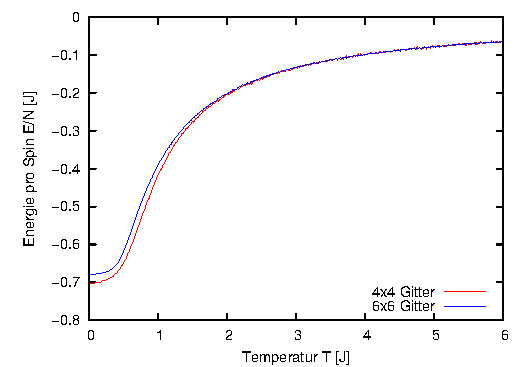
\includegraphics[width=0.48\textwidth]{Diagrams/SSE/Lattice_Energy-Temperature} 
  }
  \subfloat[{\bfseries Mittelwerte der W�rmekapazit�t}]{
    \label{fig:GitterWaermekapazitaetTemperatur}
    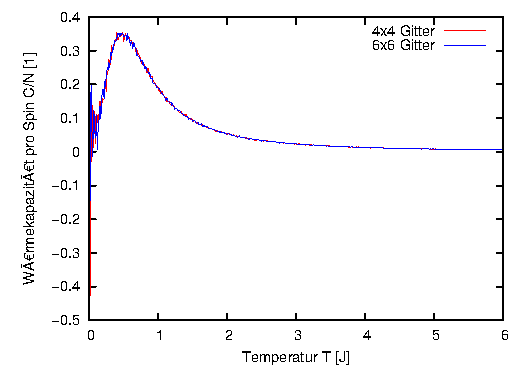
\includegraphics[width=0.48\textwidth]{Diagrams/SSE/Lattice_SpecificHeat-Temperature} 
  }
  \caption[Mittelwerte der Energie und W�rmekapazit�t; {\itshape Quelle:} Eigenwerk]{Mittelwerte der Energie und W�rmekapazit�t f�r verschiedene Systemgr��en eines periodischen Gitters bei 100000 Messpunkten pro Temperaturpunkt; {\itshape Quelle:} Eigenwerk}
  \label{fig:ModellEnergieWaermekapazitaet}
\end{figure}

\subsection{Vergleich verschiedener Modelle / Exakte Diagonalisierung}

In den Abbildungen \ref{fig:AlleEnergieTemperatur} und \ref{fig:AlleWaermekapazitaetTemperatur} sind die Energie und die W�rmekapazit�t f�r die drei betrachteten Modelle (Kette mit offenen, Kette mit periodischen und Gitter mit periodischen Randbedingungen) aufgetragen. Die exakte, dunklere Linie beschreibt die Werte der ED-Methode {\itshape(Exakte Diagonalisierung)}.

Die Energiekurven zeigen im 1-dimensionalen Fall keinen sichtbaren Unterschied zwischen den Methoden SSE und ED, wohingegen die SSE-Werte f�r das Gitter eine gut sichtbare h�here Ungenauigkeit aufweisen. Die Differenz der Grundzustandsenergien erkl�ren sich wohl Haupts�chlich durch die gr��ere Anzahl von Koppelungen pro Spin, qualitativ zeigen die Kurven allerdings ebenfalls kaum Unterschiede.

Die Ableitung der Energie nach der Temperatur, die W�rmekapazit�t, ist wie erwartet deutlich ungenauer. Besonders in den Temperaturen nahe 0 spielen arithmetische Fehler der Implementierung (Maschinengenauigkeit) eine gro�e Rolle, da dort gro�e Zahlen subtrahiert werden. Auffallend ist, dass die beiden periodischen Modelle diesselbe maximale W�rmekapazit�t besitzen.

\begin{figure}[bh]
  \centering
  \subfloat[{\bfseries Mittelwerte der Energie}]{
    \label{fig:AlleEnergieTemperatur}
    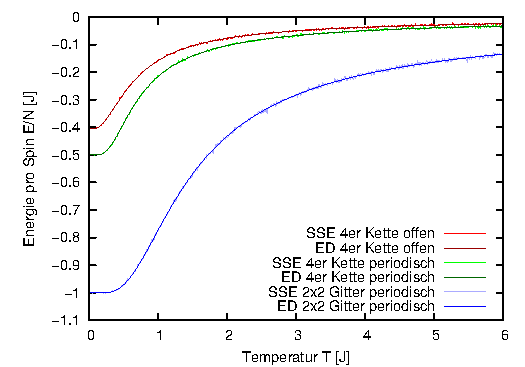
\includegraphics[width=0.48\textwidth]{Diagrams/SSE/All_Energy-Temperature} 
  }
  \subfloat[{\bfseries Mittelwerte der W�rmekapazit�t}]{
    \label{fig:AlleWaermekapazitaetTemperatur}
    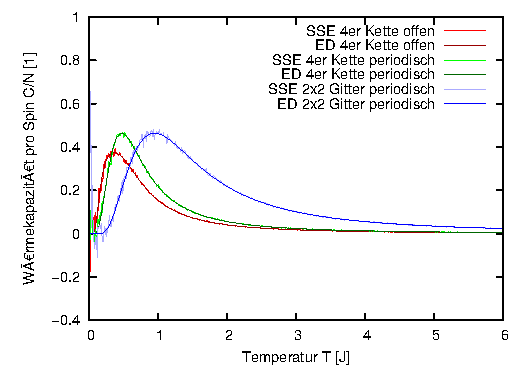
\includegraphics[width=0.48\textwidth]{Diagrams/SSE/All_SpecificHeat-Temperature} 
  }
  \caption[Mittelwerte der Energie und W�rmekapazit�t; {\itshape Quelle:} Eigenwerk]{Mittelwerte der Energie und W�rmekapazit�t f�r die verschiedenen Modelle 1D-Offen, 1-Periodisch und 2D-Periodisch mit der Spinanzahl 4 bei 100000 Messpunkten pro Temperaturpunkt; {\itshape Quelle:} Eigenwerk}
  \label{fig:AlleEnergieWaermekapazitaet}
\end{figure}

An dem Beispiel der 4 Spin langen Heisenbergkette mit offenen Randbedingungen, wollen wir uns nun noch die Verwendung der Exakten Diagonalisierung veranschaulichen \cite{Ham}:

Da der Hamiltonian jeden Unter-Zustandsraum $\Omega_i$ aller Basiszust�nde diesselbe Anzahl $i$ aufw�rtsgerichteter Spins (siehe \cite{Spincount}) stabil l�sst (Erhaltung der Summe aller $S_j^z$), stellt er in einer geeignet sortierten Basis eine Blockmatrix dar:

\tiny
\[
H=\left(\begin{blockarray}{cccccccccccccccc}
\begin{block}{\{c\}ccccccccccccccc}
0.75  &&&&&&&&&&&&&&& 0\\
\end{block}
\begin{block}{c\{cccc\}ccccccccccc}
& 0.25  & 0.5   & 0     & 0     \\
& 0.5   & -0.25 & 0.5   & 0     \\
& 0     & 0.5   & -0.25 & 0.5   \\
& 0     & 0     & 0.5   & 0.25  \\
\end{block}
\begin{block}{ccccc\{cccccc\}ccccc}
&&&&& 0.25  & 0.5   & 0     & 0     & 0     & 0     \\
&&&&& 0.5   & -0.75 & 0.5   & 0.5   & 0     & 0     \\
&&&&& 0     & 0.5   & -0.25 & 0     & 0.5   & 0     \\
&&&&& 0     & 0.5   & 0     & -0.25 & 0.5   & 0     \\
&&&&& 0     & 0     & 0.5   & 0.5   & -0.75 & 0.5   \\
&&&&& 0     & 0     & 0     & 0     & 0.5   & 0.25  \\
\end{block}
\begin{block}{ccccccccccc\{cccc\}c}
&&&&&&&&&&& 0.25  & 0.5   & 0     & 0     \\
&&&&&&&&&&& 0.5   & -0.25 & 0.5   & 0     \\
&&&&&&&&&&& 0     & 0.5   & -0.25 & 0.5   \\
&&&&&&&&&&& 0     & 0     & 0.5   & 0.25  \\
\end{block}
\begin{block}{ccccccccccccccc\{c\}}
0&&&&&&&&&&&&&&& 0.75  \\
\end{block}
\end{blockarray}\right)
\]
\normalsize

Die Bl�cke k�nnen nun einzeln diagonalisiert werden, was einen deutlichen Performancegewinn gegen�ber einer gesamten Diagonalisierung darstellt. Die Eigenwerte der obigen Matrix sind \{0.75, 0.75, 0.75, 0.75, 0.75, 0.457107, 0.457107, 0.457107, 0.116025, -0.25, -0.25, -0.25, -0.957107, -0.957107, -0.957107, -1.61603\}. Mithilfe dieser k�nnen nun z.B. die Boltzmanngewichte bzw. die Zustandssumme berechnet werden.

\newpage
\thispagestyle{empty}
\cleardoublepage
\chapter{Zusammenfassung}

Die {\bfseries Stochastic Series Expansion} stellt ein m�chtiges Werkzeug f�r das Sampling von Operatorstrings innerhalb eines quantenmechanischen L�sungsansatzes dar. Sie ist f�r gr��ere 2-dimensionale Systeme der schnellste Weg, um die typischen, thermodynamischen Gr��en zu messen und wird hierf�r an mehreren Instituten erfolgreich eingesetzt. Der Algorithmus ist relativ leicht zu implementieren und arbeitet �u�erst speichersparend.

Im Rahmen dieser Arbeit wurde ein Simulationsprogramm geschrieben, welches nicht nur ein blo�es SSE Modul enth�lt, sondern die M�glichkeit anbietet, die SSE-Daten f�r kleine Systeme mit ED {\bfseries Exakt Diagonalisation} zu �berpr�fen, dar�ber hinaus kann ein Zusatzmodul f�r das numerische L�sen des klassischen Ising-Modells eingesetzt werden. Da das Sofware-Projekt objekt-orientiert ausgelegt ist, k�nnen beliebige Komponenten, wie mit einem Baukastensystem zusammengestellt werden. Es ist dadurch sehr flexibel.

Die durchgef�hrten Messungen best�tigten stets die Theorie und liefern besitzen nur einen sehr geringen Fehler. 

Physikalische Sachverhalte werden an mehreren Beispielen/Bildern erkl�hrt und die Abschnitte "`Methode"' in den beiden Projektskapitel 3 und 4 f�hren ausf�hrliche Beschreibungen der 3 Algorithmen an.

\appendix

\newpage
\thispagestyle{empty}
\cleardoublepage
\chapter{Quellcode}
\label{sec:code}

\section{Hauptprogramm SIM}

\cppcodefile[label=code:SIM]{SIM.cpp}

\section{Gitter Klassen}

\subsection{Abstrakte Gitterklasse}

\cppcodefile[label=code:AbstractLattice]{Classes/Lattice/AbstractLattice.cpp}

\subsection{1D Gitter mit offenen Randbedingungen}

\cppcodefile[label=code:Open1DLattice]{Classes/Lattice/Open1DLattice.cpp}

\subsection{1D Gitter mit periodischen Randbedingungen}

\cppcodefile[label=code:Periodic1DLattice]{Classes/Lattice/Periodic1DLattice.cpp}

\subsection{2D Gitter mit periodischen Randbedingungen}

\cppcodefile[label=code:Periodic2DLattice]{Classes/Lattice/Periodic2DLattice.cpp}

\section{Algorithmus Klassen}

\subsection{Abstrakte Algorithmusklasse}

\cppcodefile[label=code:AbstractAlgorithm]{Classes/Algorithm/AbstractAlgorithm.cpp}

\subsection{ED Algorithmus}

\cppcodefile[label=code:EDAlgorithm]{Classes/Algorithm/EDAlgorithm.cpp}

\subsection{Ising Algorithmus}

\cppcodefile[label=code:ISINGAlgorithm]{Classes/Algorithm/ISINGAlgorithm.cpp}

\subsection{SSE Algorithmus}

\cppcodefile[label=code:SSEAlgorithm]{Classes/Algorithm/SSEAlgorithm.cpp}

\section{Analysemodule}

\subsection{Abstrakte Analyseklasse}

\cppcodefile[label=code:AbstractAnalyzer]{Classes/Analyzer/AbstractAnalyzer.cpp}

\subsection{Analyse f�r die Energie (Ising)}

\cppcodefile[label=code:IsingEnergyAnalyzer]{Classes/Analyzer/IsingEnergyAnalyzer.cpp}

\subsection{Analyse f�r die W�rmekapazit�t (Ising)}

\cppcodefile[label=code:IsingHeatCapacityAnalyzer]{Classes/Analyzer/IsingHeatCapacityAnalyzer.cpp}

\subsection{Analyse f�r die Magnetisierung (Ising)}

\cppcodefile[label=code:IsingMagnetisationAnalyzer]{Classes/Analyzer/IsingMagnetisationAnalyzer.cpp}

\subsection{Analyse f�r die magnetische Suszeptibilit�t (Ising)}

\cppcodefile[label=code:IsingSusceptibilityAnalyzer]{Classes/Analyzer/IsingSusceptibilityAnalyzer.cpp}

\subsection{Analyse f�r die abs. Magnetisierung (Ising)}

\cppcodefile[label=code:IsingAbsoluteMagnetisationAnalyzer]{Classes/Analyzer/IsingAbsoluteMagnetisationAnalyzer.cpp}

\subsection{Analyse f�r die abs. mag. Suszeptibilit�t (Ising)}

\cppcodefile[label=code:IsingAbsoluteSusceptibilityAnalyzer]{Classes/Analyzer/IsingAbsoluteSusceptibilityAnalyzer.cpp}

\subsection{Analyse f�r die Energie (SSE)}

\cppcodefile[label=code:SseEnergyAnalyzer]{Classes/Analyzer/SseEnergyAnalyzer.cpp}

\subsection{Analyse f�r die W�rmekapazit�t (SSE)}

\cppcodefile[label=code:SseHeatCapacityAnalyzer]{Classes/Analyzer/SseHeatCapacityAnalyzer.cpp}

%=======================================

\newpage
\thispagestyle{empty}
\cleardoublepage
\let\listfigurenamePARENT\listfigurename
\renewcommand{\listfigurename}{\addcontentsline{toc}{chapter}{\listfigurenamePARENT}\listfigurenamePARENT}
\begingroup
\renewcommand*{\addvspace}[1]{}
\listoffigures
\endgroup

\newpage
\thispagestyle{empty}
\cleardoublepage
\renewcommand{\lstlistlistingname}{\addcontentsline{toc}{chapter}{Quellcodeverzeichnis}Quellcodeverzeichnis}
\lstlistoflistings

\newpage
\thispagestyle{empty}
\cleardoublepage
\let\bibnamePARENT\bibname
\renewcommand{\bibname}{\addcontentsline{toc}{chapter}{\bibnamePARENT}\bibnamePARENT}
\bibliographystyle{alphadin}
\bibliography{Literature}

\newpage
\thispagestyle{empty}
\cleardoublepage
\chapter*{Erkl�rung zur Selbstst�ndigkeit}
\addcontentsline{toc}{chapter}{Erkl�hrung zur Selbstst�ndigkeit}

Hiermit versichere ich, dass ich diese Arbeit selbstst�ndig verfasst und keine anderen als die angegebenen Quellen und Hilfsmittel benutzt habe.

\vspace{10mm}
\begin{tabular}{@{}p{40mm}@{\hspace{1mm}}l@{\hspace{1mm}}p{30mm}@{\hspace{6mm}}p{50mm}}
\hrule&,&\hrule&\hrule\\[-3mm]
Ort&&Datum&Unterschrift\\
\end{tabular}

\end{document}